% Options for packages loaded elsewhere
% Options for packages loaded elsewhere
\PassOptionsToPackage{unicode}{hyperref}
\PassOptionsToPackage{hyphens}{url}
\PassOptionsToPackage{dvipsnames,svgnames,x11names}{xcolor}
%
\documentclass[
  letterpaper,
  DIV=11,
  numbers=noendperiod]{scrartcl}
\usepackage{xcolor}
\usepackage{amsmath,amssymb}
\setcounter{secnumdepth}{-\maxdimen} % remove section numbering
\usepackage{iftex}
\ifPDFTeX
  \usepackage[T1]{fontenc}
  \usepackage[utf8]{inputenc}
  \usepackage{textcomp} % provide euro and other symbols
\else % if luatex or xetex
  \usepackage{unicode-math} % this also loads fontspec
  \defaultfontfeatures{Scale=MatchLowercase}
  \defaultfontfeatures[\rmfamily]{Ligatures=TeX,Scale=1}
\fi
\usepackage{lmodern}
\ifPDFTeX\else
  % xetex/luatex font selection
\fi
% Use upquote if available, for straight quotes in verbatim environments
\IfFileExists{upquote.sty}{\usepackage{upquote}}{}
\IfFileExists{microtype.sty}{% use microtype if available
  \usepackage[]{microtype}
  \UseMicrotypeSet[protrusion]{basicmath} % disable protrusion for tt fonts
}{}
\makeatletter
\@ifundefined{KOMAClassName}{% if non-KOMA class
  \IfFileExists{parskip.sty}{%
    \usepackage{parskip}
  }{% else
    \setlength{\parindent}{0pt}
    \setlength{\parskip}{6pt plus 2pt minus 1pt}}
}{% if KOMA class
  \KOMAoptions{parskip=half}}
\makeatother
% Make \paragraph and \subparagraph free-standing
\makeatletter
\ifx\paragraph\undefined\else
  \let\oldparagraph\paragraph
  \renewcommand{\paragraph}{
    \@ifstar
      \xxxParagraphStar
      \xxxParagraphNoStar
  }
  \newcommand{\xxxParagraphStar}[1]{\oldparagraph*{#1}\mbox{}}
  \newcommand{\xxxParagraphNoStar}[1]{\oldparagraph{#1}\mbox{}}
\fi
\ifx\subparagraph\undefined\else
  \let\oldsubparagraph\subparagraph
  \renewcommand{\subparagraph}{
    \@ifstar
      \xxxSubParagraphStar
      \xxxSubParagraphNoStar
  }
  \newcommand{\xxxSubParagraphStar}[1]{\oldsubparagraph*{#1}\mbox{}}
  \newcommand{\xxxSubParagraphNoStar}[1]{\oldsubparagraph{#1}\mbox{}}
\fi
\makeatother

\usepackage{color}
\usepackage{fancyvrb}
\newcommand{\VerbBar}{|}
\newcommand{\VERB}{\Verb[commandchars=\\\{\}]}
\DefineVerbatimEnvironment{Highlighting}{Verbatim}{commandchars=\\\{\}}
% Add ',fontsize=\small' for more characters per line
\usepackage{framed}
\definecolor{shadecolor}{RGB}{241,243,245}
\newenvironment{Shaded}{\begin{snugshade}}{\end{snugshade}}
\newcommand{\AlertTok}[1]{\textcolor[rgb]{0.68,0.00,0.00}{#1}}
\newcommand{\AnnotationTok}[1]{\textcolor[rgb]{0.37,0.37,0.37}{#1}}
\newcommand{\AttributeTok}[1]{\textcolor[rgb]{0.40,0.45,0.13}{#1}}
\newcommand{\BaseNTok}[1]{\textcolor[rgb]{0.68,0.00,0.00}{#1}}
\newcommand{\BuiltInTok}[1]{\textcolor[rgb]{0.00,0.23,0.31}{#1}}
\newcommand{\CharTok}[1]{\textcolor[rgb]{0.13,0.47,0.30}{#1}}
\newcommand{\CommentTok}[1]{\textcolor[rgb]{0.37,0.37,0.37}{#1}}
\newcommand{\CommentVarTok}[1]{\textcolor[rgb]{0.37,0.37,0.37}{\textit{#1}}}
\newcommand{\ConstantTok}[1]{\textcolor[rgb]{0.56,0.35,0.01}{#1}}
\newcommand{\ControlFlowTok}[1]{\textcolor[rgb]{0.00,0.23,0.31}{\textbf{#1}}}
\newcommand{\DataTypeTok}[1]{\textcolor[rgb]{0.68,0.00,0.00}{#1}}
\newcommand{\DecValTok}[1]{\textcolor[rgb]{0.68,0.00,0.00}{#1}}
\newcommand{\DocumentationTok}[1]{\textcolor[rgb]{0.37,0.37,0.37}{\textit{#1}}}
\newcommand{\ErrorTok}[1]{\textcolor[rgb]{0.68,0.00,0.00}{#1}}
\newcommand{\ExtensionTok}[1]{\textcolor[rgb]{0.00,0.23,0.31}{#1}}
\newcommand{\FloatTok}[1]{\textcolor[rgb]{0.68,0.00,0.00}{#1}}
\newcommand{\FunctionTok}[1]{\textcolor[rgb]{0.28,0.35,0.67}{#1}}
\newcommand{\ImportTok}[1]{\textcolor[rgb]{0.00,0.46,0.62}{#1}}
\newcommand{\InformationTok}[1]{\textcolor[rgb]{0.37,0.37,0.37}{#1}}
\newcommand{\KeywordTok}[1]{\textcolor[rgb]{0.00,0.23,0.31}{\textbf{#1}}}
\newcommand{\NormalTok}[1]{\textcolor[rgb]{0.00,0.23,0.31}{#1}}
\newcommand{\OperatorTok}[1]{\textcolor[rgb]{0.37,0.37,0.37}{#1}}
\newcommand{\OtherTok}[1]{\textcolor[rgb]{0.00,0.23,0.31}{#1}}
\newcommand{\PreprocessorTok}[1]{\textcolor[rgb]{0.68,0.00,0.00}{#1}}
\newcommand{\RegionMarkerTok}[1]{\textcolor[rgb]{0.00,0.23,0.31}{#1}}
\newcommand{\SpecialCharTok}[1]{\textcolor[rgb]{0.37,0.37,0.37}{#1}}
\newcommand{\SpecialStringTok}[1]{\textcolor[rgb]{0.13,0.47,0.30}{#1}}
\newcommand{\StringTok}[1]{\textcolor[rgb]{0.13,0.47,0.30}{#1}}
\newcommand{\VariableTok}[1]{\textcolor[rgb]{0.07,0.07,0.07}{#1}}
\newcommand{\VerbatimStringTok}[1]{\textcolor[rgb]{0.13,0.47,0.30}{#1}}
\newcommand{\WarningTok}[1]{\textcolor[rgb]{0.37,0.37,0.37}{\textit{#1}}}

\usepackage{longtable,booktabs,array}
\usepackage{calc} % for calculating minipage widths
% Correct order of tables after \paragraph or \subparagraph
\usepackage{etoolbox}
\makeatletter
\patchcmd\longtable{\par}{\if@noskipsec\mbox{}\fi\par}{}{}
\makeatother
% Allow footnotes in longtable head/foot
\IfFileExists{footnotehyper.sty}{\usepackage{footnotehyper}}{\usepackage{footnote}}
\makesavenoteenv{longtable}
\usepackage{graphicx}
\makeatletter
\newsavebox\pandoc@box
\newcommand*\pandocbounded[1]{% scales image to fit in text height/width
  \sbox\pandoc@box{#1}%
  \Gscale@div\@tempa{\textheight}{\dimexpr\ht\pandoc@box+\dp\pandoc@box\relax}%
  \Gscale@div\@tempb{\linewidth}{\wd\pandoc@box}%
  \ifdim\@tempb\p@<\@tempa\p@\let\@tempa\@tempb\fi% select the smaller of both
  \ifdim\@tempa\p@<\p@\scalebox{\@tempa}{\usebox\pandoc@box}%
  \else\usebox{\pandoc@box}%
  \fi%
}
% Set default figure placement to htbp
\def\fps@figure{htbp}
\makeatother





\setlength{\emergencystretch}{3em} % prevent overfull lines

\providecommand{\tightlist}{%
  \setlength{\itemsep}{0pt}\setlength{\parskip}{0pt}}



 


\KOMAoption{captions}{tableheading}
\makeatletter
\@ifpackageloaded{caption}{}{\usepackage{caption}}
\AtBeginDocument{%
\ifdefined\contentsname
  \renewcommand*\contentsname{Table of contents}
\else
  \newcommand\contentsname{Table of contents}
\fi
\ifdefined\listfigurename
  \renewcommand*\listfigurename{List of Figures}
\else
  \newcommand\listfigurename{List of Figures}
\fi
\ifdefined\listtablename
  \renewcommand*\listtablename{List of Tables}
\else
  \newcommand\listtablename{List of Tables}
\fi
\ifdefined\figurename
  \renewcommand*\figurename{Figure}
\else
  \newcommand\figurename{Figure}
\fi
\ifdefined\tablename
  \renewcommand*\tablename{Table}
\else
  \newcommand\tablename{Table}
\fi
}
\@ifpackageloaded{float}{}{\usepackage{float}}
\floatstyle{ruled}
\@ifundefined{c@chapter}{\newfloat{codelisting}{h}{lop}}{\newfloat{codelisting}{h}{lop}[chapter]}
\floatname{codelisting}{Listing}
\newcommand*\listoflistings{\listof{codelisting}{List of Listings}}
\makeatother
\makeatletter
\makeatother
\makeatletter
\@ifpackageloaded{caption}{}{\usepackage{caption}}
\@ifpackageloaded{subcaption}{}{\usepackage{subcaption}}
\makeatother
\usepackage{bookmark}
\IfFileExists{xurl.sty}{\usepackage{xurl}}{} % add URL line breaks if available
\urlstyle{same}
\hypersetup{
  pdftitle={Part 1: Data Cleaning and Analysis},
  colorlinks=true,
  linkcolor={blue},
  filecolor={Maroon},
  citecolor={Blue},
  urlcolor={Blue},
  pdfcreator={LaTeX via pandoc}}


\title{Part 1: Data Cleaning and Analysis}
\author{}
\date{}
\begin{document}
\maketitle


This notebook walks through the process of cleaning a human resources
dataset and performing exploratory data analysis (EDA). The goal is to
prepare the data for future modeling tasks and extract useful insights
from key HR metrics.

\subsection{Step 1: Import Required
Libraries}\label{step-1-import-required-libraries}

We begin by importing all necessary Python libraries such as: -
\texttt{pandas} and \texttt{numpy} for data manipulation - \texttt{os}
for file path management - \texttt{plotly.express} for interactive
visualizations

\begin{Shaded}
\begin{Highlighting}[]
\ImportTok{import}\NormalTok{ pandas }\ImportTok{as}\NormalTok{ pd}
\ImportTok{import}\NormalTok{ numpy }\ImportTok{as}\NormalTok{ np }
\ImportTok{import}\NormalTok{ os}
\ImportTok{import}\NormalTok{ plotly.express }\ImportTok{as}\NormalTok{ px}
\end{Highlighting}
\end{Shaded}

\begin{Shaded}
\begin{Highlighting}[]
\CommentTok{\#get working directory}
\NormalTok{current\_dir }\OperatorTok{=}\NormalTok{ os.getcwd()}

\CommentTok{\# Go one directory up to the root directory}
\NormalTok{project\_root\_dir }\OperatorTok{=}\NormalTok{ os.path.dirname(current\_dir)}

\CommentTok{\#define paths to the data folders}
\NormalTok{data\_dir }\OperatorTok{=}\NormalTok{ os.path.join(project\_root\_dir,}\StringTok{\textquotesingle{}data\textquotesingle{}}\NormalTok{)}
\NormalTok{raw\_dir }\OperatorTok{=}\NormalTok{ os.path.join(data\_dir,}\StringTok{\textquotesingle{}raw\textquotesingle{}}\NormalTok{)}
\NormalTok{processed\_dir }\OperatorTok{=}\NormalTok{ os.path.join(data\_dir,}\StringTok{\textquotesingle{}processed\textquotesingle{}}\NormalTok{) }

\CommentTok{\# define path results folder }
\NormalTok{results\_dir }\OperatorTok{=}\NormalTok{ os.path.join(project\_root\_dir,}\StringTok{\textquotesingle{}results\textquotesingle{}}\NormalTok{)}

\CommentTok{\# define paths to docs folder}
\NormalTok{docs\_dir }\OperatorTok{=}\NormalTok{ os.path.join(project\_root\_dir,}\StringTok{\textquotesingle{}docs\textquotesingle{}}\NormalTok{)}

\CommentTok{\# Create directories if they do not exit}
\NormalTok{os.makedirs(raw\_dir, exist\_ok }\OperatorTok{=} \VariableTok{True}\NormalTok{) }
\NormalTok{os.makedirs(processed\_dir, exist\_ok }\OperatorTok{=} \VariableTok{True}\NormalTok{) }
\NormalTok{os.makedirs(results\_dir, exist\_ok }\OperatorTok{=} \VariableTok{True}\NormalTok{)}
\NormalTok{os.makedirs(docs\_dir, exist\_ok }\OperatorTok{=} \VariableTok{True}\NormalTok{)}
\end{Highlighting}
\end{Shaded}

\subsection{Step 2: Load the Dataset}\label{step-2-load-the-dataset}

We load the cleaned CSV file containing employee data. This step also
includes checking the first few rows to confirm successful import.

\begin{Shaded}
\begin{Highlighting}[]
\NormalTok{HR\_Analytics\_filename }\OperatorTok{=}\NormalTok{ os.path.join(processed\_dir, }\StringTok{"HR\_Analytics.csv"}\NormalTok{)}
\NormalTok{HR\_Analytics\_df }\OperatorTok{=}\NormalTok{ pd.read\_csv(HR\_Analytics\_filename)}
\NormalTok{HR\_Analytics\_df.head(}\DecValTok{10}\NormalTok{)}
\end{Highlighting}
\end{Shaded}

\subsection{Step 3: Explore Dataset
Structure}\label{step-3-explore-dataset-structure}

Before we begin cleaning, it's essential to understand the overall
structure and condition of our dataset. This step helps us identify
potential issues such as missing values, irrelevant columns, or
inconsistent data types.

We use the following methods:

.shape This method returns a tuple containing the number of rows and
columns in the dataset.

\begin{Shaded}
\begin{Highlighting}[]
\NormalTok{HR\_Analytics\_df.shape}
\end{Highlighting}
\end{Shaded}

\begin{verbatim}
(1473, 39)
\end{verbatim}

\subsection{.info()}\label{info}

This method gives a concise summary of the DataFrame including: - Column
names - Data types (e.g., \texttt{int64}, \texttt{object},
\texttt{float64}) - Non-null counts (how many values are present) -
Memory usage

This is especially useful for: - Identifying columns with missing values
(by comparing non-null count to total rows) - Detecting incorrect data
types (e.g., numbers stored as strings)

\begin{Shaded}
\begin{Highlighting}[]
\NormalTok{HR\_Analytics\_df.info()}
\end{Highlighting}
\end{Shaded}

\begin{verbatim}
<class 'pandas.core.frame.DataFrame'>
RangeIndex: 1473 entries, 0 to 1472
Data columns (total 39 columns):
 #   Column                          Non-Null Count  Dtype 
---  ------                          --------------  ----- 
 0   EmpID                           1473 non-null   object
 1   Age                             1473 non-null   int64 
 2   AgeGroup                        1473 non-null   object
 3   Attrition                       1473 non-null   object
 4   BusinessTravel                  1473 non-null   object
 5   DailyRate                       1473 non-null   int64 
 6   Department                      1473 non-null   object
 7   DistanceFromHome                1473 non-null   int64 
 8   Education                       1473 non-null   int64 
 9   EducationField                  1473 non-null   object
 10  EnvSatisfaction                 1473 non-null   int64 
 11  Gender                          1473 non-null   object
 12  HourlyRate                      1473 non-null   int64 
 13  JobInvolvement                  1473 non-null   int64 
 14  JobLevel                        1473 non-null   int64 
 15  JobRole                         1473 non-null   object
 16  JobSatisfaction                 1473 non-null   int64 
 17  MaritalStatus                   1473 non-null   object
 18  MonthlyIncome                   1473 non-null   int64 
 19  MonthlyRate                     1473 non-null   int64 
 20  NumCompaniesWorked              1473 non-null   int64 
 21  OverTime                        1473 non-null   object
 22  PercentSalaryHike               1473 non-null   int64 
 23  PerformanceRating               1473 non-null   int64 
 24  RelationshipSatisfaction        1473 non-null   int64 
 25  StockOptionLevel                1473 non-null   int64 
 26  TotalWorkingYears               1473 non-null   int64 
 27  TrainingTimesLastYear           1473 non-null   int64 
 28  WorkLifeBalance                 1473 non-null   int64 
 29  YearsAtCompany                  1473 non-null   int64 
 30  YearsInCurrentRole              1473 non-null   int64 
 31  YearsSinceLastPromotion         1473 non-null   int64 
 32  YearsWithCurrManager            1473 non-null   object
 33  Education_Level                 1473 non-null   object
 34  JobLevelLabel                   1473 non-null   object
 35  JobInvolveLabel                 1473 non-null   object
 36  StockOptionLevel_Description    1473 non-null   object
 37  RelationshipSatisfaction_Label  1473 non-null   object
 38  WorkLifeLabel                   1473 non-null   object
dtypes: int64(22), object(17)
memory usage: 448.9+ KB
\end{verbatim}

\subsection{.isnull().sum()}\label{isnull.sum}

This function checks for missing values in each column and counts how
many there are.\\
It helps us pinpoint exactly which columns require imputation or
cleaning.\\
Columns with zero missing values are fine, while columns with non-zero
values may need intervention.

This structural exploration ensures we are aware of any data quality
issues before proceeding with transformations or analysis.

\begin{Shaded}
\begin{Highlighting}[]
\NormalTok{HR\_Analytics\_df.isnull().}\BuiltInTok{sum}\NormalTok{()}
\end{Highlighting}
\end{Shaded}

\begin{verbatim}
EmpID                             0
Age                               0
AgeGroup                          0
Attrition                         0
BusinessTravel                    0
DailyRate                         0
Department                        0
DistanceFromHome                  0
Education                         0
EducationField                    0
EnvSatisfaction                   0
Gender                            0
HourlyRate                        0
JobInvolvement                    0
JobLevel                          0
JobRole                           0
JobSatisfaction                   0
MaritalStatus                     0
MonthlyIncome                     0
MonthlyRate                       0
NumCompaniesWorked                0
OverTime                          0
PercentSalaryHike                 0
PerformanceRating                 0
RelationshipSatisfaction          0
StockOptionLevel                  0
TotalWorkingYears                 0
TrainingTimesLastYear             0
WorkLifeBalance                   0
YearsAtCompany                    0
YearsInCurrentRole                0
YearsSinceLastPromotion           0
YearsWithCurrManager              0
Education_Level                   0
JobLevelLabel                     0
JobInvolveLabel                   0
StockOptionLevel_Description      0
RelationshipSatisfaction_Label    0
WorkLifeLabel                     0
dtype: int64
\end{verbatim}

\subsection{Step 4: Handling Missing
Values}\label{step-4-handling-missing-values}

In this step, we address missing data. For example, the
\texttt{YearsWithCurrManager} column is filled with a placeholder value
(``unknown'') where nulls exist. This ensures consistency and prevents
issues during analysis or modeling.

\begin{Shaded}
\begin{Highlighting}[]
\NormalTok{HR\_Analytics\_df[}\StringTok{\textquotesingle{}YearsWithCurrManager\textquotesingle{}}\NormalTok{]}\OperatorTok{=}\NormalTok{HR\_Analytics\_df[}\StringTok{\textquotesingle{}YearsWithCurrManager\textquotesingle{}}\NormalTok{].fillna(}\StringTok{\textquotesingle{}unknown\textquotesingle{}}\NormalTok{)}
\end{Highlighting}
\end{Shaded}

\begin{Shaded}
\begin{Highlighting}[]
\NormalTok{HR\_Analytics\_df.isnull().}\BuiltInTok{sum}\NormalTok{()}
\end{Highlighting}
\end{Shaded}

\begin{verbatim}
EmpID                             0
Age                               0
AgeGroup                          0
Attrition                         0
BusinessTravel                    0
DailyRate                         0
Department                        0
DistanceFromHome                  0
Education                         0
EducationField                    0
EnvSatisfaction                   0
Gender                            0
HourlyRate                        0
JobInvolvement                    0
JobLevel                          0
JobRole                           0
JobSatisfaction                   0
MaritalStatus                     0
MonthlyIncome                     0
MonthlyRate                       0
NumCompaniesWorked                0
OverTime                          0
PercentSalaryHike                 0
PerformanceRating                 0
RelationshipSatisfaction          0
StockOptionLevel                  0
TotalWorkingYears                 0
TrainingTimesLastYear             0
WorkLifeBalance                   0
YearsAtCompany                    0
YearsInCurrentRole                0
YearsSinceLastPromotion           0
YearsWithCurrManager              0
Education_Level                   0
JobLevelLabel                     0
JobInvolveLabel                   0
StockOptionLevel_Description      0
RelationshipSatisfaction_Label    0
WorkLifeLabel                     0
dtype: int64
\end{verbatim}

\subsection{Step 5: Remove Duplicate
Rows}\label{step-5-remove-duplicate-rows}

We check for any duplicated rows in the dataset and drop them if found.
Removing duplicates ensures that statistical analysis is not biased by
repeated records.

\begin{Shaded}
\begin{Highlighting}[]
\NormalTok{HR\_Analytics\_df.duplicated().}\BuiltInTok{sum}\NormalTok{()}
\end{Highlighting}
\end{Shaded}

\begin{verbatim}
0
\end{verbatim}

\begin{Shaded}
\begin{Highlighting}[]
\NormalTok{HR\_Analytics\_df[HR\_Analytics\_df.duplicated(keep}\OperatorTok{=}\VariableTok{False}\NormalTok{)]}
\end{Highlighting}
\end{Shaded}

\begin{longtable}[]{@{}llllllllllllllllllllll@{}}
\toprule\noalign{}
& EmpID & Age & AgeGroup & Attrition & BusinessTravel & DailyRate &
Department & DistanceFromHome & Education & EducationField & ... &
YearsAtCompany & YearsInCurrentRole & YearsSinceLastPromotion &
YearsWithCurrManager & Education\_Level & JobLevelLabel &
JobInvolveLabel & StockOptionLevel\_Description &
RelationshipSatisfaction\_Label & WorkLifeLabel \\
\midrule\noalign{}
\endhead
\bottomrule\noalign{}
\endlastfoot
\end{longtable}

\subsubsection{Removing Duplicate
Records}\label{removing-duplicate-records}

In this step, we remove any duplicate rows from the dataset using the
\texttt{.drop\_duplicates()} method.

\begin{itemize}
\tightlist
\item
  Duplicate records occur when the same combination of values appears in
  multiple rows. This can result from errors during data entry, merging
  datasets, or exporting from systems.
\item
  Keeping duplicates can lead to biased analysis, especially in
  aggregate statistics or machine learning models, since repeated rows
  are treated as separate, valid observations.
\item
  This removes all fully duplicated rows (i.e., rows where every column
  matches another row).
\end{itemize}

\begin{Shaded}
\begin{Highlighting}[]
\NormalTok{HR\_Analytics\_df}\OperatorTok{=}\NormalTok{ HR\_Analytics\_df.drop\_duplicates()}
\end{Highlighting}
\end{Shaded}

The result is stored back into the original DataFrame to ensure we're
working with only unique records going forward.

Now can verify how many duplicates were removed by checking:

\begin{Shaded}
\begin{Highlighting}[]
\NormalTok{HR\_Analytics\_df.duplicated().}\BuiltInTok{sum}\NormalTok{()}
\end{Highlighting}
\end{Shaded}

\begin{verbatim}
0
\end{verbatim}

\begin{Shaded}
\begin{Highlighting}[]
\NormalTok{HR\_Analytics\_df.shape}
\end{Highlighting}
\end{Shaded}

\begin{verbatim}
(1473, 39)
\end{verbatim}

\subsubsection{Identifying Categorical (Object-Type)
Columns}\label{identifying-categorical-object-type-columns}

Before performing encoding or feature transformations, it's important to
identify which columns in the dataset are considered categorical (i.e.,
non-numeric). In pandas, these are typically stored as \texttt{object}
data types. .dtypes returns the data type of each column in the
DataFrame.

By comparing this to object, we create a Boolean Series:

True for columns that are stored as object type (usually strings or
mixed types)

False for numeric columns (e.g., int64, float64)

This helps us:

Identify which columns may need encoding for machine learning (e.g.,
label encoding, one-hot encoding).

Detect data quality issues, such as numeric columns that are incorrectly
stored as strings.

Plan feature engineering (e.g., transforming string-based fields like
Department, JobRole, or Education into categorical codes).

To see just the names of those columns, you can extend this:

\begin{Shaded}
\begin{Highlighting}[]
\NormalTok{HR\_Analytics\_df.dtypes }\OperatorTok{==} \BuiltInTok{object}
\end{Highlighting}
\end{Shaded}

\begin{verbatim}
EmpID                              True
Age                               False
AgeGroup                           True
Attrition                          True
BusinessTravel                     True
DailyRate                         False
Department                         True
DistanceFromHome                  False
Education                         False
EducationField                     True
EnvSatisfaction                   False
Gender                             True
HourlyRate                        False
JobInvolvement                    False
JobLevel                          False
JobRole                            True
JobSatisfaction                   False
MaritalStatus                      True
MonthlyIncome                     False
MonthlyRate                       False
NumCompaniesWorked                False
OverTime                           True
PercentSalaryHike                 False
PerformanceRating                 False
RelationshipSatisfaction          False
StockOptionLevel                  False
TotalWorkingYears                 False
TrainingTimesLastYear             False
WorkLifeBalance                   False
YearsAtCompany                    False
YearsInCurrentRole                False
YearsSinceLastPromotion           False
YearsWithCurrManager               True
Education_Level                    True
JobLevelLabel                      True
JobInvolveLabel                    True
StockOptionLevel_Description       True
RelationshipSatisfaction_Label     True
WorkLifeLabel                      True
dtype: bool
\end{verbatim}

This filtered view is very useful during preprocessing.

\begin{Shaded}
\begin{Highlighting}[]
\CommentTok{\#HR\_Analytics.drop(columns=[\textquotesingle{}Over18\textquotesingle{}, \textquotesingle{}SalarySlab\textquotesingle{}, \textquotesingle{}EmployeeCount\textquotesingle{}, \textquotesingle{}StandardHours\textquotesingle{}, \textquotesingle{}EmployeeNumber\textquotesingle{}], inplace= True)}
\end{Highlighting}
\end{Shaded}

\subsubsection{Displaying All Column
Names}\label{displaying-all-column-names}

When working with a dataset, it's helpful to quickly view all the column
names. This gives us an overview of the available features and allows us
to plan our cleaning or analysis steps.

\begin{Shaded}
\begin{Highlighting}[]
\NormalTok{HR\_Analytics\_df.columns}
\end{Highlighting}
\end{Shaded}

\begin{verbatim}
Index(['EmpID', 'Age', 'AgeGroup', 'Attrition', 'BusinessTravel', 'DailyRate',
       'Department', 'DistanceFromHome', 'Education', 'EducationField',
       'EnvSatisfaction', 'Gender', 'HourlyRate', 'JobInvolvement', 'JobLevel',
       'JobRole', 'JobSatisfaction', 'MaritalStatus', 'MonthlyIncome',
       'MonthlyRate', 'NumCompaniesWorked', 'OverTime', 'PercentSalaryHike',
       'PerformanceRating', 'RelationshipSatisfaction', 'StockOptionLevel',
       'TotalWorkingYears', 'TrainingTimesLastYear', 'WorkLifeBalance',
       'YearsAtCompany', 'YearsInCurrentRole', 'YearsSinceLastPromotion',
       'YearsWithCurrManager', 'Education_Level', 'JobLevelLabel',
       'JobInvolveLabel', 'StockOptionLevel_Description',
       'RelationshipSatisfaction_Label', 'WorkLifeLabel'],
      dtype='object')
\end{verbatim}

\subsection{This returns an Index object containing the names of all
columns in the
DataFrame.}\label{this-returns-an-index-object-containing-the-names-of-all-columns-in-the-dataframe.}

It's especially useful when:

You want to check for typos or inconsistencies in column names.

You're selecting specific columns for transformation or analysis.

You're about to drop, rename, or reorder columns.

This method provides a clean and fast way to understand the dataset's
structure from a feature (column) perspective --- especially when the
dataset has many columns that don't all fit on screen in .head() or
.info() views.

\begin{Shaded}
\begin{Highlighting}[]
\NormalTok{HR\_Analytics\_df.shape}
\end{Highlighting}
\end{Shaded}

\begin{verbatim}
(1473, 39)
\end{verbatim}

\begin{Shaded}
\begin{Highlighting}[]
\NormalTok{HR\_Analytics\_df.columns}
\end{Highlighting}
\end{Shaded}

\begin{verbatim}
Index(['EmpID', 'Age', 'AgeGroup', 'Attrition', 'BusinessTravel', 'DailyRate',
       'Department', 'DistanceFromHome', 'Education', 'EducationField',
       'EnvSatisfaction', 'Gender', 'HourlyRate', 'JobInvolvement', 'JobLevel',
       'JobRole', 'JobSatisfaction', 'MaritalStatus', 'MonthlyIncome',
       'MonthlyRate', 'NumCompaniesWorked', 'OverTime', 'PercentSalaryHike',
       'PerformanceRating', 'RelationshipSatisfaction', 'StockOptionLevel',
       'TotalWorkingYears', 'TrainingTimesLastYear', 'WorkLifeBalance',
       'YearsAtCompany', 'YearsInCurrentRole', 'YearsSinceLastPromotion',
       'YearsWithCurrManager', 'Education_Level', 'JobLevelLabel',
       'JobInvolveLabel', 'StockOptionLevel_Description',
       'RelationshipSatisfaction_Label', 'WorkLifeLabel'],
      dtype='object')
\end{verbatim}

By running .unique(), we can:

Confirm whether all expected education levels are present.

Detect unexpected or invalid entries (e.g., values outside the 1--5
range).

Decide how to transform these values --- for instance, mapping the codes
to human-readable labels using a dictionary.

This step is part of feature exploration and validation before
performing any transformations or analysis.

\begin{Shaded}
\begin{Highlighting}[]
\NormalTok{HR\_Analytics\_df[}\StringTok{\textquotesingle{}Education\textquotesingle{}}\NormalTok{].unique()}
\end{Highlighting}
\end{Shaded}

\begin{verbatim}
array([3, 2, 1, 4, 5], dtype=int64)
\end{verbatim}

\subsubsection{Exploring Unique Values in the `Education'
Column}\label{exploring-unique-values-in-the-education-column}

Before transforming or analyzing a column, it's important to understand
what values it contains. We use \texttt{.unique()} to inspect all
distinct entries in a column.

\begin{verbatim}
This line does the following:
\end{verbatim}

Accesses the Education column in the dataset.

Returns an array of unique values found in that column.

Helps us understand the range of categories or codes being used.

In the HR dataset, the Education column stores numeric codes that
represent different levels of education, such as:

\begin{longtable}[]{@{}ll@{}}
\toprule\noalign{}
code & Meaning \\
\midrule\noalign{}
\endhead
\bottomrule\noalign{}
\endlastfoot
1 & Below College \\
2 & college \\
3 & Bachelor \\
4 & Masters \\
5 & Doctors \\
\end{longtable}

\begin{Shaded}
\begin{Highlighting}[]
\NormalTok{education\_map }\OperatorTok{=}\NormalTok{ \{}
    \DecValTok{1}\NormalTok{: }\StringTok{\textquotesingle{}Below College\textquotesingle{}}\NormalTok{,}
    \DecValTok{2}\NormalTok{: }\StringTok{\textquotesingle{}College\textquotesingle{}}\NormalTok{,}
    \DecValTok{3}\NormalTok{: }\StringTok{\textquotesingle{}Bachelor\textquotesingle{}}\NormalTok{,}
    \DecValTok{4}\NormalTok{: }\StringTok{\textquotesingle{}Master\textquotesingle{}}\NormalTok{,}
    \DecValTok{5}\NormalTok{: }\StringTok{\textquotesingle{}Doctor\textquotesingle{}}
\NormalTok{\}}
\end{Highlighting}
\end{Shaded}

\begin{Shaded}
\begin{Highlighting}[]
\NormalTok{HR\_Analytics\_df[}\StringTok{\textquotesingle{}Education\_Level\textquotesingle{}}\NormalTok{] }\OperatorTok{=}\NormalTok{ HR\_Analytics\_df[}\StringTok{\textquotesingle{}Education\textquotesingle{}}\NormalTok{].}\BuiltInTok{map}\NormalTok{(education\_map) }
\end{Highlighting}
\end{Shaded}

\begin{Shaded}
\begin{Highlighting}[]
\NormalTok{HR\_Analytics\_df[}\StringTok{\textquotesingle{}Education\_Level\textquotesingle{}}\NormalTok{].unique()}
\end{Highlighting}
\end{Shaded}

\begin{verbatim}
array(['Bachelor', 'College', 'Below College', 'Master', 'Doctor'],
      dtype=object)
\end{verbatim}

\subsection{Renaming a Column for
Simplicity}\label{renaming-a-column-for-simplicity}

To make column names shorter and easier to work with, we rename the
\texttt{EnvironmentSatisfaction} column to \texttt{EnvSatisfaction}.
rename(columns=\{\ldots\}): Specifies which column(s) to rename.

`EnvironmentSatisfaction': `EnvSatisfaction': Renames the long column
name to a shorter one.

inplace=True: Applies the change directly to the DataFrame without
needing to assign it again.

This helps make code cleaner and easier to read

\begin{Shaded}
\begin{Highlighting}[]
\NormalTok{HR\_Analytics\_df.rename(columns}\OperatorTok{=}\NormalTok{\{}\StringTok{\textquotesingle{}EnvironmentSatisfaction\textquotesingle{}}\NormalTok{: }\StringTok{\textquotesingle{}EnvSatisfaction\textquotesingle{}}\NormalTok{\}, inplace}\OperatorTok{=}\VariableTok{True}\NormalTok{)}
\end{Highlighting}
\end{Shaded}

\subsection{Checking Unique Values in the JobLevel
Column}\label{checking-unique-values-in-the-joblevel-column}

We use \texttt{.unique()} to identify all distinct job level values in
the dataset.

\begin{Shaded}
\begin{Highlighting}[]
\NormalTok{HR\_Analytics\_df[}\StringTok{\textquotesingle{}JobLevel\textquotesingle{}}\NormalTok{].unique()}
\end{Highlighting}
\end{Shaded}

\begin{verbatim}
array([1, 2, 3, 4, 5], dtype=int64)
\end{verbatim}

\subsection{Exploring Unique Job
Levels}\label{exploring-unique-job-levels}

To understand the range of job seniority levels in the dataset, we check
the unique values in the \texttt{JobLevel} column. Each number
corresponds to a specific level in the job hierarchy: \textbar{} code
\textbar{} Meaning \textbar{}
\textbar:-----------\textbar:----------\textbar{} \textbar{} 1
\textbar Entry Level\textbar{} \textbar{} 2 \textbar{} Junior
Level\textbar{} \textbar{} 3 \textbar{} Mid Level\textbar{} \textbar{} 4
\textbar{} Senior Level\textbar{} \textbar{} 5 \textbar{} Executive
Level\textbar{}

This step helps us interpret the data better and is useful for grouping
or filtering employees based on seniority.

\begin{Shaded}
\begin{Highlighting}[]
\NormalTok{job\_level\_map }\OperatorTok{=}\NormalTok{ \{}
    \DecValTok{1}\NormalTok{: }\StringTok{\textquotesingle{}Junior\textquotesingle{}}\NormalTok{,}
    \DecValTok{2}\NormalTok{: }\StringTok{\textquotesingle{}Intermediate\textquotesingle{}}\NormalTok{,}
    \DecValTok{3}\NormalTok{: }\StringTok{\textquotesingle{}Senior\textquotesingle{}}\NormalTok{,}
    \DecValTok{4}\NormalTok{: }\StringTok{\textquotesingle{}Manager\textquotesingle{}}\NormalTok{,}
    \DecValTok{5}\NormalTok{: }\StringTok{\textquotesingle{}Senior Executive\textquotesingle{}}
\NormalTok{\}}
\end{Highlighting}
\end{Shaded}

\begin{Shaded}
\begin{Highlighting}[]
\NormalTok{HR\_Analytics\_df[}\StringTok{\textquotesingle{}JobLevelLabel\textquotesingle{}}\NormalTok{] }\OperatorTok{=}\NormalTok{ HR\_Analytics\_df[}\StringTok{\textquotesingle{}JobLevel\textquotesingle{}}\NormalTok{].}\BuiltInTok{map}\NormalTok{(job\_level\_map)}
\end{Highlighting}
\end{Shaded}

\begin{Shaded}
\begin{Highlighting}[]
\NormalTok{HR\_Analytics\_df[}\StringTok{\textquotesingle{}JobLevelLabel\textquotesingle{}}\NormalTok{].unique()}
\end{Highlighting}
\end{Shaded}

\begin{verbatim}
array(['Junior', 'Intermediate', 'Senior', 'Manager', 'Senior Executive'],
      dtype=object)
\end{verbatim}

\subsection{Checking Unique Values in the JobInvolvement
Column}\label{checking-unique-values-in-the-jobinvolvement-column}

To understand the range of job involvement scores in the dataset, we use
the \texttt{.unique()} function:

\begin{Shaded}
\begin{Highlighting}[]
\NormalTok{HR\_Analytics\_df[}\StringTok{\textquotesingle{}JobInvolvement\textquotesingle{}}\NormalTok{].unique()}
\end{Highlighting}
\end{Shaded}

\begin{verbatim}
array([3, 2, 1, 4], dtype=int64)
\end{verbatim}

\subsection{Creating a Mapping for Job Involvement
Levels}\label{creating-a-mapping-for-job-involvement-levels}

We define a dictionary called \texttt{job\_involve\_map} to translate
the numeric values in the \texttt{JobInvolvement} column into meaningful
text labels.

In the dataset, JobInvolvement uses numbers (1 to 4) to rate how engaged
an employee is in their job.

This dictionary maps each number to a corresponding descriptive label:
\textbar{} code \textbar{} Meaning \textbar{}
\textbar:-----------\textbar:----------\textbar{} \textbar{} 1
\textbar Low\textbar{} \textbar{} 2 \textbar{} Medium\textbar{}
\textbar{} 3 \textbar{} High\textbar{} \textbar{} 4 \textbar{} Very
High\textbar{}

This mapping helps make the data more understandable when visualizing or
reporting on employee involvement.

\begin{Shaded}
\begin{Highlighting}[]
\NormalTok{job\_involve\_map }\OperatorTok{=}\NormalTok{ \{}
    \DecValTok{1}\NormalTok{: }\StringTok{\textquotesingle{}Low\textquotesingle{}}\NormalTok{,}
    \DecValTok{2}\NormalTok{: }\StringTok{\textquotesingle{}Medium\textquotesingle{}}\NormalTok{,}
    \DecValTok{3}\NormalTok{: }\StringTok{\textquotesingle{}High\textquotesingle{}}\NormalTok{,}
    \DecValTok{4}\NormalTok{: }\StringTok{\textquotesingle{}Very High\textquotesingle{}}
\NormalTok{\}}
\end{Highlighting}
\end{Shaded}

\subsection{Mapping Job Involvement Scores to
Labels}\label{mapping-job-involvement-scores-to-labels}

We create a new column called \texttt{JobInvolveLabel} by mapping the
numeric values in the \texttt{JobInvolvement} column to descriptive
labels using a dictionary called \texttt{job\_level\_map}.

\begin{Shaded}
\begin{Highlighting}[]
\NormalTok{HR\_Analytics\_df[}\StringTok{\textquotesingle{}JobInvolveLabel\textquotesingle{}}\NormalTok{] }\OperatorTok{=}\NormalTok{ HR\_Analytics\_df[}\StringTok{\textquotesingle{}JobInvolvement\textquotesingle{}}\NormalTok{].}\BuiltInTok{map}\NormalTok{(job\_level\_map)}
\end{Highlighting}
\end{Shaded}

\begin{Shaded}
\begin{Highlighting}[]
\NormalTok{HR\_Analytics\_df[}\StringTok{\textquotesingle{}JobInvolveLabel\textquotesingle{}}\NormalTok{].unique()}
\end{Highlighting}
\end{Shaded}

\begin{verbatim}
array(['Senior', 'Intermediate', 'Junior', 'Manager'], dtype=object)
\end{verbatim}

\begin{Shaded}
\begin{Highlighting}[]
\NormalTok{HR\_Analytics\_df[}\StringTok{\textquotesingle{}JobSatisfaction\textquotesingle{}}\NormalTok{].unique()}
\end{Highlighting}
\end{Shaded}

\begin{verbatim}
array([3, 2, 4, 1], dtype=int64)
\end{verbatim}

\begin{Shaded}
\begin{Highlighting}[]
\CommentTok{\#job\_satisfaction\_map = \{}
    \CommentTok{\#1: \textquotesingle{}Poor\textquotesingle{},}
    \CommentTok{\#2: \textquotesingle{}Fair\textquotesingle{},}
    \CommentTok{\#3: \textquotesingle{}Good\textquotesingle{},}
    \CommentTok{\#4: \textquotesingle{}Very Good\textquotesingle{}}
\CommentTok{\#\}}
\end{Highlighting}
\end{Shaded}

\begin{Shaded}
\begin{Highlighting}[]
\CommentTok{\#HR\_Analytics.rename(columns=\{\textquotesingle{}JobSatisfaction\textquotesingle{}: \textquotesingle{}JobSatisfy\_Level\textquotesingle{}\}, inplace=True)}
\CommentTok{\#HR\_Analytics[\textquotesingle{}JobSatisfy\_Label\textquotesingle{}] = HR\_Analytics[\textquotesingle{}JobSatisfy\_Level\textquotesingle{}].map(job\_satisfaction\_map)}
\end{Highlighting}
\end{Shaded}

\begin{Shaded}
\begin{Highlighting}[]
\CommentTok{\#HR\_Analytics[\textquotesingle{}JobSatisfy\_Label\textquotesingle{}].unique()}
\end{Highlighting}
\end{Shaded}

\begin{Shaded}
\begin{Highlighting}[]
\CommentTok{\#HR\_Analytics[\textquotesingle{}PerformanceRating\textquotesingle{}].unique()}
\end{Highlighting}
\end{Shaded}

\begin{Shaded}
\begin{Highlighting}[]
\CommentTok{\#performance\_score\_map = \{}
    \CommentTok{\#3: \textquotesingle{}Good\textquotesingle{},}
    \CommentTok{\#4: \textquotesingle{}Excellent\textquotesingle{}}
\CommentTok{\#\}}
\end{Highlighting}
\end{Shaded}

\begin{Shaded}
\begin{Highlighting}[]
\CommentTok{\#HR\_Analytics.rename(columns=\{\textquotesingle{}PerformanceRating\textquotesingle{}: \textquotesingle{}PerformanceScore\textquotesingle{}\}, inplace=True)}
\end{Highlighting}
\end{Shaded}

\begin{Shaded}
\begin{Highlighting}[]
\CommentTok{\#HR\_Analytics[\textquotesingle{}PerformanceLabel\textquotesingle{}] = HR\_Analytics[\textquotesingle{}PerformanceScore\textquotesingle{}].map(performance\_score\_map)}
\end{Highlighting}
\end{Shaded}

\begin{Shaded}
\begin{Highlighting}[]
\CommentTok{\#HR\_Analytics[\textquotesingle{}PerformanceLabel\textquotesingle{}].unique()}
\end{Highlighting}
\end{Shaded}

\subsection{Checking Unique Values in the StockOptionLevel
Column}\label{checking-unique-values-in-the-stockoptionlevel-column}

To see the different levels of stock options offered to employees, we
use the \texttt{.unique()} function:

\begin{Shaded}
\begin{Highlighting}[]
\NormalTok{HR\_Analytics\_df[}\StringTok{\textquotesingle{}StockOptionLevel\textquotesingle{}}\NormalTok{].unique()}
\end{Highlighting}
\end{Shaded}

\begin{verbatim}
array([0, 2, 1, 3], dtype=int64)
\end{verbatim}

\subsection{Mapping Stock Option Levels to
Descriptions}\label{mapping-stock-option-levels-to-descriptions}

We define a dictionary to convert numeric stock option levels into
descriptive labels, then create a new column with these descriptions.

\begin{longtable}[]{@{}ll@{}}
\toprule\noalign{}
code & Meaning \\
\midrule\noalign{}
\endhead
\bottomrule\noalign{}
\endlastfoot
0 & No stock options \\
1 & Low stock options \\
2 & Medium stock options \\
3 & High stock options \\
\end{longtable}

The StockOptionLevel column contains numeric codes representing the
level of stock options granted to employees.

Using .map() with stock\_option\_map, we translate these codes into
human-readable labels.

The new column StockOptionLevel\_Description stores these descriptive
labels, making the data easier to interpret in reports and
visualizations.

\begin{Shaded}
\begin{Highlighting}[]
\NormalTok{stock\_option\_map }\OperatorTok{=}\NormalTok{ \{}
    \DecValTok{0}\NormalTok{: }\StringTok{\textquotesingle{}No Stock Options\textquotesingle{}}\NormalTok{,}
    \DecValTok{1}\NormalTok{: }\StringTok{\textquotesingle{}Low Stock Options\textquotesingle{}}\NormalTok{,}
    \DecValTok{2}\NormalTok{: }\StringTok{\textquotesingle{}Medium Stock Options\textquotesingle{}}\NormalTok{,}
    \DecValTok{3}\NormalTok{: }\StringTok{\textquotesingle{}High Stock Options\textquotesingle{}}
\NormalTok{\}}

\NormalTok{HR\_Analytics\_df[}\StringTok{\textquotesingle{}StockOptionLevel\_Description\textquotesingle{}}\NormalTok{] }\OperatorTok{=}\NormalTok{ HR\_Analytics\_df[}\StringTok{\textquotesingle{}StockOptionLevel\textquotesingle{}}\NormalTok{].}\BuiltInTok{map}\NormalTok{(stock\_option\_map)}
\end{Highlighting}
\end{Shaded}

\subsection{Checking Unique Values in
StockOptionLevel\_Description}\label{checking-unique-values-in-stockoptionlevel_description}

After mapping, we check the distinct descriptive labels in the
\texttt{StockOptionLevel\_Description} column

Purpose: This confirms all categories of stock options are present and
correctly labeled, making it easier to analyze employee benefits related
to stock options.

\begin{Shaded}
\begin{Highlighting}[]
\NormalTok{HR\_Analytics\_df[}\StringTok{\textquotesingle{}StockOptionLevel\_Description\textquotesingle{}}\NormalTok{].unique()}
\end{Highlighting}
\end{Shaded}

\begin{verbatim}
array(['No Stock Options', 'Medium Stock Options', 'Low Stock Options',
       'High Stock Options'], dtype=object)
\end{verbatim}

\begin{Shaded}
\begin{Highlighting}[]
\CommentTok{\#HR\_Analytics[\textquotesingle{}TrainingTimesLastYear\textquotesingle{}].unique()}
\end{Highlighting}
\end{Shaded}

\begin{Shaded}
\begin{Highlighting}[]
\CommentTok{\#training\_map = \{}
 \CommentTok{\#0: \textquotesingle{}No Training\textquotesingle{},}
  \CommentTok{\#  1: \textquotesingle{}Few\textquotesingle{},}
   \CommentTok{\# 2: \textquotesingle{}Moderate\textquotesingle{},}
    \CommentTok{\#3: \textquotesingle{}Good\textquotesingle{},}
    \CommentTok{\#4: \textquotesingle{}Very Good\textquotesingle{},}
    \CommentTok{\#5: \textquotesingle{}Excellent\textquotesingle{},}
    \CommentTok{\#6: \textquotesingle{}Exceptional\textquotesingle{}}
\CommentTok{\#\}}
\CommentTok{\#HR\_Analytics[\textquotesingle{}TrainingsLastYear\_Label\textquotesingle{}] = HR\_Analytics[\textquotesingle{}TrainingTimesLastYear\textquotesingle{}].map(training\_map)}
\end{Highlighting}
\end{Shaded}

\begin{Shaded}
\begin{Highlighting}[]
\CommentTok{\#HR\_Analytics[\textquotesingle{}TrainingsLastYear\_Label\textquotesingle{}].unique()}
\end{Highlighting}
\end{Shaded}

\subsection{Checking Unique Values in the RelationshipSatisfaction
Column}\label{checking-unique-values-in-the-relationshipsatisfaction-column}

To identify the different satisfaction levels employees have with their
relationships at work, we use the \texttt{.unique()} function:

\begin{Shaded}
\begin{Highlighting}[]
\NormalTok{HR\_Analytics\_df[}\StringTok{\textquotesingle{}RelationshipSatisfaction\textquotesingle{}}\NormalTok{].unique()}
\end{Highlighting}
\end{Shaded}

\begin{verbatim}
array([3, 1, 4, 2], dtype=int64)
\end{verbatim}

\subsection{Creating a Mapping for Relationship Satisfaction
Levels}\label{creating-a-mapping-for-relationship-satisfaction-levels}

We define a dictionary \texttt{relation\_map} to convert numeric
satisfaction scores into descriptive labels. \textbar{} code \textbar{}
Meaning \textbar{} \textbar:-----------\textbar:----------\textbar{}
\textbar{} 1 \textbar Low\textbar{} \textbar{} 2 \textbar{}
Medium\textbar{} \textbar{} 3 \textbar{} High\textbar{} \textbar{} 4
\textbar{} Very High\textbar{} The RelationshipSatisfaction column uses
numbers 1 to 4 to rate how satisfied employees are with their workplace
relationships.

This dictionary maps each number to a meaningful label, making data
easier to understand in reports and visualizations.

\begin{Shaded}
\begin{Highlighting}[]
\NormalTok{relation\_map }\OperatorTok{=}\NormalTok{ \{}
    \DecValTok{1}\NormalTok{: }\StringTok{\textquotesingle{}Low\textquotesingle{}}\NormalTok{,}
    \DecValTok{2}\NormalTok{: }\StringTok{\textquotesingle{}Medium\textquotesingle{}}\NormalTok{,}
    \DecValTok{3}\NormalTok{: }\StringTok{\textquotesingle{}High\textquotesingle{}}\NormalTok{,}
    \DecValTok{4}\NormalTok{: }\StringTok{\textquotesingle{}Very High\textquotesingle{}}
\NormalTok{\}}
\end{Highlighting}
\end{Shaded}

\subsection{Mapping Relationship Satisfaction Scores to
Labels}\label{mapping-relationship-satisfaction-scores-to-labels}

We create a new column \texttt{RelationshipSatisfaction\_Label} by
mapping numeric scores in \texttt{RelationshipSatisfaction} to
descriptive labels using the \texttt{relation\_map} dictionary.

\begin{Shaded}
\begin{Highlighting}[]
\NormalTok{HR\_Analytics\_df[}\StringTok{\textquotesingle{}RelationshipSatisfaction\_Label\textquotesingle{}}\NormalTok{] }\OperatorTok{=}\NormalTok{ HR\_Analytics\_df[}\StringTok{\textquotesingle{}RelationshipSatisfaction\textquotesingle{}}\NormalTok{].}\BuiltInTok{map}\NormalTok{(relation\_map)}
\end{Highlighting}
\end{Shaded}

\subsection{Checking Unique Values in
RelationshipSatisfaction\_Label}\label{checking-unique-values-in-relationshipsatisfaction_label}

After mapping numeric scores to descriptive labels, we check the
distinct values in the \texttt{RelationshipSatisfaction\_Label} column

\begin{Shaded}
\begin{Highlighting}[]
\NormalTok{HR\_Analytics\_df[}\StringTok{\textquotesingle{}RelationshipSatisfaction\_Label\textquotesingle{}}\NormalTok{].unique()}
\end{Highlighting}
\end{Shaded}

\begin{verbatim}
array(['High', 'Low', 'Very High', 'Medium'], dtype=object)
\end{verbatim}

\subsection{Checking Unique Values in the WorkLifeBalance
Column}\label{checking-unique-values-in-the-worklifebalance-column}

To explore the range of work-life balance ratings in the dataset, we use
the \texttt{.unique()} function.

\begin{Shaded}
\begin{Highlighting}[]
\NormalTok{HR\_Analytics\_df[}\StringTok{\textquotesingle{}WorkLifeBalance\textquotesingle{}}\NormalTok{].unique()}
\end{Highlighting}
\end{Shaded}

\begin{verbatim}
array([3, 4, 1, 2], dtype=int64)
\end{verbatim}

\subsection{Creating a Mapping for Work-Life Balance
Ratings}\label{creating-a-mapping-for-work-life-balance-ratings}

We define a dictionary called \texttt{work\_life\_map} to convert the
numeric work-life balance ratings into descriptive labels. The
WorkLifeBalance column contains numeric scores from 1 to 4.

\begin{longtable}[]{@{}ll@{}}
\toprule\noalign{}
code & Meaning \\
\midrule\noalign{}
\endhead
\bottomrule\noalign{}
\endlastfoot
1 & Poor \\
2 & Fair \\
3 & Good \\
4 & Excellent \\
\end{longtable}

This mapping translates the values into more meaningful labels Using
this dictionary helps make the dataset easier to interpret and improves
the clarity of visualizations and reports.

\begin{Shaded}
\begin{Highlighting}[]
\NormalTok{work\_life\_map }\OperatorTok{=}\NormalTok{ \{}
    \DecValTok{1}\NormalTok{: }\StringTok{\textquotesingle{}Poor\textquotesingle{}}\NormalTok{,}
    \DecValTok{2}\NormalTok{: }\StringTok{\textquotesingle{}Fair\textquotesingle{}}\NormalTok{,}
    \DecValTok{3}\NormalTok{: }\StringTok{\textquotesingle{}Good\textquotesingle{}}\NormalTok{,}
    \DecValTok{4}\NormalTok{: }\StringTok{\textquotesingle{}Excellent\textquotesingle{}}
\NormalTok{\}}
\end{Highlighting}
\end{Shaded}

Mapping Work-Life Balance Scores to Descriptive Labels

We create a new column \texttt{WorkLifeLabel} by mapping the numeric
values in the \texttt{WorkLifeBalance} column to readable labels using
the \texttt{work\_life\_map} dictionary.

\begin{Shaded}
\begin{Highlighting}[]
\NormalTok{HR\_Analytics\_df[}\StringTok{\textquotesingle{}WorkLifeLabel\textquotesingle{}}\NormalTok{] }\OperatorTok{=}\NormalTok{ HR\_Analytics\_df[}\StringTok{\textquotesingle{}WorkLifeBalance\textquotesingle{}}\NormalTok{].}\BuiltInTok{map}\NormalTok{(work\_life\_map)}
\end{Highlighting}
\end{Shaded}

Checking Unique Values in WorkLifeLabel

After mapping work-life balance scores to descriptive labels, we check
the unique values in the \texttt{WorkLifeLabel} column.

\begin{Shaded}
\begin{Highlighting}[]
\NormalTok{HR\_Analytics\_df[}\StringTok{\textquotesingle{}WorkLifeLabel\textquotesingle{}}\NormalTok{].unique()}
\end{Highlighting}
\end{Shaded}

\begin{verbatim}
array(['Good', 'Excellent', 'Poor', 'Fair'], dtype=object)
\end{verbatim}

\begin{Shaded}
\begin{Highlighting}[]
\NormalTok{HR\_Analytics\_df.columns}
\end{Highlighting}
\end{Shaded}

\begin{verbatim}
Index(['EmpID', 'Age', 'AgeGroup', 'Attrition', 'BusinessTravel', 'DailyRate',
       'Department', 'DistanceFromHome', 'Education', 'EducationField',
       'EnvSatisfaction', 'Gender', 'HourlyRate', 'JobInvolvement', 'JobLevel',
       'JobRole', 'JobSatisfaction', 'MaritalStatus', 'MonthlyIncome',
       'MonthlyRate', 'NumCompaniesWorked', 'OverTime', 'PercentSalaryHike',
       'PerformanceRating', 'RelationshipSatisfaction', 'StockOptionLevel',
       'TotalWorkingYears', 'TrainingTimesLastYear', 'WorkLifeBalance',
       'YearsAtCompany', 'YearsInCurrentRole', 'YearsSinceLastPromotion',
       'YearsWithCurrManager', 'Education_Level', 'JobLevelLabel',
       'JobInvolveLabel', 'StockOptionLevel_Description',
       'RelationshipSatisfaction_Label', 'WorkLifeLabel'],
      dtype='object')
\end{verbatim}

\begin{Shaded}
\begin{Highlighting}[]
\CommentTok{\#HR\_Analytics\_df.to\_csv("cleaned1\_HR.csv", index=False)}
\end{Highlighting}
\end{Shaded}

\begin{Shaded}
\begin{Highlighting}[]
\CommentTok{\#HR\_Analytics}
\end{Highlighting}
\end{Shaded}

\begin{Shaded}
\begin{Highlighting}[]
\CommentTok{\#HR\_Analytics.drop(}
 \CommentTok{\#   [\textquotesingle{}Education\textquotesingle{}, \textquotesingle{}JobLevel\textquotesingle{}, \textquotesingle{}JobInvolvement\textquotesingle{}, \textquotesingle{}StockOptionLevel\textquotesingle{},}
  \CommentTok{\#3    \textquotesingle{}RelationshipSatisfaction\textquotesingle{}, \textquotesingle{}WorkLifeBalance\textquotesingle{}],}
    \CommentTok{\#axis=1,}
    \CommentTok{\#errors=\textquotesingle{}ignore\textquotesingle{},}
   \CommentTok{\# inplace=True}
\CommentTok{\#)}
\end{Highlighting}
\end{Shaded}

\begin{Shaded}
\begin{Highlighting}[]
\NormalTok{HR\_Analytics\_df.columns}
\end{Highlighting}
\end{Shaded}

\begin{verbatim}
Index(['EmpID', 'Age', 'AgeGroup', 'Attrition', 'BusinessTravel', 'DailyRate',
       'Department', 'DistanceFromHome', 'Education', 'EducationField',
       'EnvSatisfaction', 'Gender', 'HourlyRate', 'JobInvolvement', 'JobLevel',
       'JobRole', 'JobSatisfaction', 'MaritalStatus', 'MonthlyIncome',
       'MonthlyRate', 'NumCompaniesWorked', 'OverTime', 'PercentSalaryHike',
       'PerformanceRating', 'RelationshipSatisfaction', 'StockOptionLevel',
       'TotalWorkingYears', 'TrainingTimesLastYear', 'WorkLifeBalance',
       'YearsAtCompany', 'YearsInCurrentRole', 'YearsSinceLastPromotion',
       'YearsWithCurrManager', 'Education_Level', 'JobLevelLabel',
       'JobInvolveLabel', 'StockOptionLevel_Description',
       'RelationshipSatisfaction_Label', 'WorkLifeLabel'],
      dtype='object')
\end{verbatim}

\begin{Shaded}
\begin{Highlighting}[]
\CommentTok{\#HR\_Analytics.to\_csv("cleaned\_HR.csv", index=False)}
\end{Highlighting}
\end{Shaded}

\subsection{Key HR Metrics Summary}\label{key-hr-metrics-summary}

We calculate and display important HR metrics to understand the overall
workforce trends in the dataset. Attrition Rate: Shows the percentage of
employees who left the company (Attrition = `Yes').

Promotion Rate: Measures the percentage of employees promoted recently
(YearsSinceLastPromotion = 0).

Performance Rating Distribution: Displays the percentage distribution of
employee performance ratings.

Average Tenure: Indicates the average number of years employees have
stayed at the company.

These metrics help assess workforce stability, growth opportunities, and
performance trends.

\begin{Shaded}
\begin{Highlighting}[]
\NormalTok{attrition\_rate }\OperatorTok{=}\NormalTok{ (HR\_Analytics\_df[}\StringTok{\textquotesingle{}Attrition\textquotesingle{}}\NormalTok{].value\_counts().get(}\StringTok{\textquotesingle{}Yes\textquotesingle{}}\NormalTok{, }\DecValTok{0}\NormalTok{) }\OperatorTok{/} \BuiltInTok{len}\NormalTok{(HR\_Analytics\_df)) }\OperatorTok{*} \DecValTok{100}
\BuiltInTok{print}\NormalTok{(}\SpecialStringTok{f"Attrition Rate: }\SpecialCharTok{\{}\NormalTok{attrition\_rate}\SpecialCharTok{:.2f\}}\SpecialStringTok{\%"}\NormalTok{)}
\end{Highlighting}
\end{Shaded}

\begin{verbatim}
Attrition Rate: 16.09%
\end{verbatim}

\begin{Shaded}
\begin{Highlighting}[]
\NormalTok{avg\_tenure }\OperatorTok{=}\NormalTok{ HR\_Analytics\_df[}\StringTok{\textquotesingle{}YearsAtCompany\textquotesingle{}}\NormalTok{].mean()}
\BuiltInTok{print}\NormalTok{(}\SpecialStringTok{f"Average Tenure: }\SpecialCharTok{\{}\NormalTok{avg\_tenure}\SpecialCharTok{:.2f\}}\SpecialStringTok{ years"}\NormalTok{)}
\end{Highlighting}
\end{Shaded}

\begin{verbatim}
Average Tenure: 7.00 years
\end{verbatim}

\begin{Shaded}
\begin{Highlighting}[]
\NormalTok{avg\_satisfaction }\OperatorTok{=}\NormalTok{ HR\_Analytics\_df[}\StringTok{\textquotesingle{}JobSatisfaction\textquotesingle{}}\NormalTok{].mean()}
\BuiltInTok{print}\NormalTok{(}\SpecialStringTok{f"Average Job Satisfaction Score: }\SpecialCharTok{\{}\NormalTok{avg\_satisfaction}\SpecialCharTok{:.2f\}}\SpecialStringTok{"}\NormalTok{)}
\end{Highlighting}
\end{Shaded}

\begin{verbatim}
Average Job Satisfaction Score: 2.73
\end{verbatim}

\begin{Shaded}
\begin{Highlighting}[]
\NormalTok{performance\_dist }\OperatorTok{=}\NormalTok{ HR\_Analytics\_df[}\StringTok{\textquotesingle{}PerformanceRating\textquotesingle{}}\NormalTok{].value\_counts(normalize}\OperatorTok{=}\VariableTok{True}\NormalTok{) }\OperatorTok{*} \DecValTok{100}
\BuiltInTok{print}\NormalTok{(performance\_dist)}
\end{Highlighting}
\end{Shaded}

\begin{verbatim}
PerformanceRating
3    84.657162
4    15.342838
Name: proportion, dtype: float64
\end{verbatim}

\begin{Shaded}
\begin{Highlighting}[]
\CommentTok{\#training\_avg = HR\_Analytics[\textquotesingle{}TrainingLastYear\_Label\textquotesingle{}].mean()}
\CommentTok{\#print(f"Average Trainings Per Employee: \{training\_avg:.2f\} times/year")}
\end{Highlighting}
\end{Shaded}

\begin{Shaded}
\begin{Highlighting}[]
\NormalTok{promoted\_count }\OperatorTok{=}\NormalTok{ (HR\_Analytics\_df[}\StringTok{\textquotesingle{}YearsSinceLastPromotion\textquotesingle{}}\NormalTok{] }\OperatorTok{==} \DecValTok{0}\NormalTok{).}\BuiltInTok{sum}\NormalTok{()}
\NormalTok{promotion\_rate }\OperatorTok{=}\NormalTok{ (promoted\_count }\OperatorTok{/} \BuiltInTok{len}\NormalTok{(HR\_Analytics\_df)) }\OperatorTok{*} \DecValTok{100}
\BuiltInTok{print}\NormalTok{(}\SpecialStringTok{f"Promotion Rate: }\SpecialCharTok{\{}\NormalTok{promotion\_rate}\SpecialCharTok{:.2f\}}\SpecialStringTok{\%"}\NormalTok{)}
\end{Highlighting}
\end{Shaded}

\begin{verbatim}
Promotion Rate: 39.58%
\end{verbatim}

\begin{Shaded}
\begin{Highlighting}[]
\NormalTok{HR\_Analytics\_df.columns}
\end{Highlighting}
\end{Shaded}

\begin{verbatim}
Index(['EmpID', 'Age', 'AgeGroup', 'Attrition', 'BusinessTravel', 'DailyRate',
       'Department', 'DistanceFromHome', 'Education', 'EducationField',
       'EnvSatisfaction', 'Gender', 'HourlyRate', 'JobInvolvement', 'JobLevel',
       'JobRole', 'JobSatisfaction', 'MaritalStatus', 'MonthlyIncome',
       'MonthlyRate', 'NumCompaniesWorked', 'OverTime', 'PercentSalaryHike',
       'PerformanceRating', 'RelationshipSatisfaction', 'StockOptionLevel',
       'TotalWorkingYears', 'TrainingTimesLastYear', 'WorkLifeBalance',
       'YearsAtCompany', 'YearsInCurrentRole', 'YearsSinceLastPromotion',
       'YearsWithCurrManager', 'Education_Level', 'JobLevelLabel',
       'JobInvolveLabel', 'StockOptionLevel_Description',
       'RelationshipSatisfaction_Label', 'WorkLifeLabel'],
      dtype='object')
\end{verbatim}

\subsection{Saving the Cleaned
Dataset}\label{saving-the-cleaned-dataset}

After cleaning and transforming the data, we save the final version to a
CSV file for future analysis or reporting. This line saves the
HR\_Analytics\_df DataFrame to a file named Cleaned1.csv.

index=False ensures that the row index is not included in the CSV file.
We can now use this cleaned dataset for visualization, reporting, or
sharing.

\begin{Shaded}
\begin{Highlighting}[]
\NormalTok{HR\_Analytics\_df.to\_csv(}\StringTok{"Cleaned1.csv"}\NormalTok{, index}\OperatorTok{=}\VariableTok{False}\NormalTok{)}
\end{Highlighting}
\end{Shaded}

This displays the final dataset, including all mapped labels and
transformed columns.

\begin{Shaded}
\begin{Highlighting}[]
\NormalTok{HR\_Analytics\_df}
\end{Highlighting}
\end{Shaded}

\begin{longtable}[]{@{}llllllllllllllllllllll@{}}
\toprule\noalign{}
& EmpID & Age & AgeGroup & Attrition & BusinessTravel & DailyRate &
Department & DistanceFromHome & Education & EducationField & ... &
YearsAtCompany & YearsInCurrentRole & YearsSinceLastPromotion &
YearsWithCurrManager & Education\_Level & JobLevelLabel &
JobInvolveLabel & StockOptionLevel\_Description &
RelationshipSatisfaction\_Label & WorkLifeLabel \\
\midrule\noalign{}
\endhead
\bottomrule\noalign{}
\endlastfoot
0 & RM297 & 18 & 18-25 & Yes & Travel\_Rarely & 230 & Research \&
Development & 3 & 3 & Life Sciences & ... & 0 & 0 & 0 & 0.0 & Bachelor &
Junior & Senior & No Stock Options & High & Good \\
1 & RM302 & 18 & 18-25 & No & Travel\_Rarely & 812 & Sales & 10 & 3 &
Medical & ... & 0 & 0 & 0 & 0.0 & Bachelor & Junior & Intermediate & No
Stock Options & Low & Good \\
2 & RM458 & 18 & 18-25 & Yes & Travel\_Frequently & 1306 & Sales & 5 & 3
& Marketing & ... & 0 & 0 & 0 & 0.0 & Bachelor & Junior & Senior & No
Stock Options & Very High & Good \\
3 & RM728 & 18 & 18-25 & No & Non-Travel & 287 & Research \& Development
& 5 & 2 & Life Sciences & ... & 0 & 0 & 0 & 0.0 & College & Junior &
Senior & No Stock Options & Very High & Good \\
4 & RM829 & 18 & 18-25 & Yes & Non-Travel & 247 & Research \&
Development & 8 & 1 & Medical & ... & 0 & 0 & 0 & 0.0 & Below College &
Junior & Senior & No Stock Options & Very High & Good \\
... & ... & ... & ... & ... & ... & ... & ... & ... & ... & ... & ... &
... & ... & ... & ... & ... & ... & ... & ... & ... & ... \\
1468 & RM412 & 60 & 55+ & No & Travel\_Rarely & 422 & Research \&
Development & 7 & 3 & Life Sciences & ... & 29 & 8 & 11 & 10.0 &
Bachelor & Senior Executive & Senior & No Stock Options & Very High &
Poor \\
1469 & RM428 & 60 & 55+ & No & Travel\_Frequently & 1499 & Sales & 28 &
3 & Marketing & ... & 18 & 13 & 13 & 11.0 & Bachelor & Senior &
Intermediate & No Stock Options & Very High & Excellent \\
1470 & RM537 & 60 & 55+ & No & Travel\_Rarely & 1179 & Sales & 16 & 4 &
Marketing & ... & 2 & 2 & 2 & 2.0 & Master & Intermediate & Senior & No
Stock Options & Very High & Good \\
1471 & RM880 & 60 & 55+ & No & Travel\_Rarely & 696 & Sales & 7 & 4 &
Marketing & ... & 11 & 7 & 1 & 9.0 & Master & Intermediate & Manager &
Low Stock Options & Medium & Good \\
1472 & RM1210 & 60 & 55+ & No & Travel\_Rarely & 370 & Research \&
Development & 1 & 4 & Medical & ... & 1 & 0 & 0 & 0.0 & Master & Senior
& Junior & Low Stock Options & High & Excellent \\
\end{longtable}

\subsection{Part 2: Data Analysis}\label{part-2-data-analysis}

\subsection{Importing Required Libraries and Visualizing Attrition Rate
by Job
Role}\label{importing-required-libraries-and-visualizing-attrition-rate-by-job-role}

Before creating visualizations, we import the necessary Python
libraries. os: Provides functions to interact with the operating system.
In our case, we use it to create folders and save visual files (like
charts).

plotly.express as px: Imports Plotly Express, a high-level API for
creating interactive and visually appealing charts such as bar charts,
line charts, and scatter plots

We use Plotly to create a grouped bar chart showing the percentage of
attrition across different job roles. This helps identify which roles
are most affected by employee turnover. The chart helps compare
attrition rates across job roles side by side.

Colors distinguish between employees who left (Yes) and those who stayed
(No).

Exporting the chart in .jpg, .png, and .html formats allows for easy
sharing and embedding into reports or dashboards.

\begin{Shaded}
\begin{Highlighting}[]
\ImportTok{import}\NormalTok{ os}
\ImportTok{import}\NormalTok{ plotly.express }\ImportTok{as}\NormalTok{ px}

\CommentTok{\# Your grouping and calculation remains the same}

\NormalTok{color\_discrete\_map }\OperatorTok{=}\NormalTok{ \{}
    \StringTok{\textquotesingle{}Yes\textquotesingle{}}\NormalTok{: }\StringTok{\textquotesingle{}\#d62728\textquotesingle{}}\NormalTok{,  }\CommentTok{\# red for attrition}
    \StringTok{\textquotesingle{}No\textquotesingle{}}\NormalTok{: }\StringTok{\textquotesingle{}\#1f77b4\textquotesingle{}}    \CommentTok{\# blue for no attrition}
\NormalTok{\}}

\NormalTok{fig }\OperatorTok{=}\NormalTok{ px.bar(}
\NormalTok{    attrition\_by\_role,}
\NormalTok{    x}\OperatorTok{=}\StringTok{\textquotesingle{}JobRole\textquotesingle{}}\NormalTok{,}
\NormalTok{    y}\OperatorTok{=}\StringTok{\textquotesingle{}percentage\textquotesingle{}}\NormalTok{,}
\NormalTok{    color}\OperatorTok{=}\StringTok{\textquotesingle{}Attrition\textquotesingle{}}\NormalTok{,}
\NormalTok{    barmode}\OperatorTok{=}\StringTok{\textquotesingle{}group\textquotesingle{}}\NormalTok{,}
\NormalTok{    title}\OperatorTok{=}\StringTok{\textquotesingle{}Attrition Rate by Job Role (\%)\textquotesingle{}}\NormalTok{,}
\NormalTok{    labels}\OperatorTok{=}\NormalTok{\{}\StringTok{\textquotesingle{}percentage\textquotesingle{}}\NormalTok{: }\StringTok{\textquotesingle{}Percentage\textquotesingle{}}\NormalTok{, }\StringTok{\textquotesingle{}JobRole\textquotesingle{}}\NormalTok{: }\StringTok{\textquotesingle{}Job Role\textquotesingle{}}\NormalTok{\},}
\NormalTok{    color\_discrete\_map}\OperatorTok{=}\NormalTok{color\_discrete\_map,}
\NormalTok{    text}\OperatorTok{=}\StringTok{\textquotesingle{}percentage\textquotesingle{}}\NormalTok{,}
\NormalTok{    width}\OperatorTok{=}\DecValTok{700}\NormalTok{,}
\NormalTok{    height}\OperatorTok{=}\DecValTok{450}
\NormalTok{)}

\NormalTok{fig.update\_layout(}
\NormalTok{    xaxis\_tickangle}\OperatorTok{=}\DecValTok{60}\NormalTok{,}
\NormalTok{    xaxis}\OperatorTok{=}\BuiltInTok{dict}\NormalTok{(automargin}\OperatorTok{=}\VariableTok{True}\NormalTok{, tickfont}\OperatorTok{=}\BuiltInTok{dict}\NormalTok{(size}\OperatorTok{=}\DecValTok{10}\NormalTok{)),}
\NormalTok{    margin}\OperatorTok{=}\BuiltInTok{dict}\NormalTok{(b}\OperatorTok{=}\DecValTok{150}\NormalTok{),}
\NormalTok{    template}\OperatorTok{=}\StringTok{"presentation"}\NormalTok{,}
\NormalTok{    paper\_bgcolor}\OperatorTok{=}\StringTok{"rgba(0,0,0,0)"}\NormalTok{,}
\NormalTok{    plot\_bgcolor}\OperatorTok{=}\StringTok{"rgba(0,0,0,0)"}\NormalTok{,}
\NormalTok{    legend\_title\_text}\OperatorTok{=}\StringTok{"Attrition"}
\NormalTok{)}

\NormalTok{fig.update\_traces(texttemplate}\OperatorTok{=}\StringTok{\textquotesingle{}\%}\SpecialCharTok{\{text:.1f\}}\StringTok{\%\textquotesingle{}}\NormalTok{, textposition}\OperatorTok{=}\StringTok{\textquotesingle{}outside\textquotesingle{}}\NormalTok{)}
\NormalTok{fig.update\_traces(}
\NormalTok{    hovertemplate}\OperatorTok{=}\StringTok{\textquotesingle{}\textless{}b\textgreater{}\%}\SpecialCharTok{\{x\}}\StringTok{\textless{}/b\textgreater{}\textless{}br\textgreater{}Attrition: \%}\SpecialCharTok{\{marker.color\}}\StringTok{\textless{}br\textgreater{}Percentage: \%}\SpecialCharTok{\{y:.2f\}}\StringTok{\%\textless{}extra\textgreater{}\textless{}/extra\textgreater{}\textquotesingle{}}
\NormalTok{)}

\NormalTok{fig.show()}

\NormalTok{results\_dir }\OperatorTok{=} \StringTok{\textquotesingle{}results\textquotesingle{}}
\NormalTok{os.makedirs(results\_dir, exist\_ok}\OperatorTok{=}\VariableTok{True}\NormalTok{)}
\NormalTok{fig.write\_image(os.path.join(results\_dir, }\StringTok{\textquotesingle{}Attrition\_Rate\_bar\_chart.jpg\textquotesingle{}}\NormalTok{))}
\NormalTok{fig.write\_image(os.path.join(results\_dir, }\StringTok{\textquotesingle{}Attrition\_Rate\_bar\_chart.png\textquotesingle{}}\NormalTok{))}
\NormalTok{fig.write\_html(os.path.join(results\_dir, }\StringTok{\textquotesingle{}Attrition\_Rate\_bar\_chart.html\textquotesingle{}}\NormalTok{))}
\end{Highlighting}
\end{Shaded}

\pandocbounded{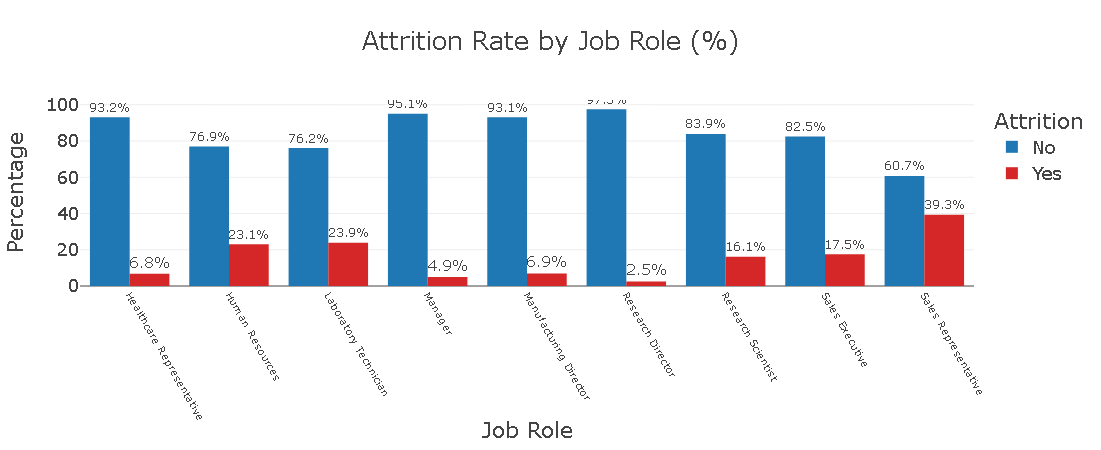
\includegraphics[keepaspectratio]{HR_Analytics_files/figure-pdf/cell-71-output-1.png}}

\subsection{Visualizing Attrition by Job
Role}\label{visualizing-attrition-by-job-role}

In this step, we analyze and visualize how employee attrition varies
across different job roles. Grouping: We group the data by JobRole and
Attrition to count how many employees left or stayed in each role.

Percentage Calculation: We calculate the percentage of attrition per job
role for meaningful comparison.

Visualization: A grouped bar chart shows the attrition percentage for
each role, using color to distinguish between employees who left (Yes)
and those who stayed (No).

Styling: Plotly's Set2 color palette and layout settings improve clarity
and presentation.

Exporting: The chart is saved in JPG, PNG, and HTML formats inside a
results/ folder, which is created if it doesn't already exist.

This chart helps HR quickly spot which job roles are experiencing higher
turnover and may need attention.

\begin{Shaded}
\begin{Highlighting}[]
\ImportTok{import}\NormalTok{ os}
\NormalTok{results\_dir }\OperatorTok{=} \StringTok{\textquotesingle{}results\textquotesingle{}}
\NormalTok{os.makedirs(results\_dir, exist\_ok}\OperatorTok{=}\VariableTok{True}\NormalTok{)}

\CommentTok{\# Group and calculate attrition percentage by JobRole}
\NormalTok{attrition\_by\_role }\OperatorTok{=}\NormalTok{ HR\_Analytics\_df.groupby([}\StringTok{\textquotesingle{}JobRole\textquotesingle{}}\NormalTok{, }\StringTok{\textquotesingle{}Attrition\textquotesingle{}}\NormalTok{]).size().reset\_index(name}\OperatorTok{=}\StringTok{\textquotesingle{}count\textquotesingle{}}\NormalTok{)}
\NormalTok{total\_per\_role }\OperatorTok{=}\NormalTok{ attrition\_by\_role.groupby(}\StringTok{\textquotesingle{}JobRole\textquotesingle{}}\NormalTok{)[}\StringTok{\textquotesingle{}count\textquotesingle{}}\NormalTok{].transform(}\StringTok{\textquotesingle{}sum\textquotesingle{}}\NormalTok{)}
\NormalTok{attrition\_by\_role[}\StringTok{\textquotesingle{}percentage\textquotesingle{}}\NormalTok{] }\OperatorTok{=} \BuiltInTok{round}\NormalTok{((attrition\_by\_role[}\StringTok{\textquotesingle{}count\textquotesingle{}}\NormalTok{] }\OperatorTok{/}\NormalTok{ total\_per\_role) }\OperatorTok{*} \DecValTok{100}\NormalTok{, }\DecValTok{2}\NormalTok{)}

\CommentTok{\# Plot}
\NormalTok{fig }\OperatorTok{=}\NormalTok{ px.bar(attrition\_by\_role,}
\NormalTok{             x}\OperatorTok{=}\StringTok{\textquotesingle{}JobRole\textquotesingle{}}\NormalTok{,}
\NormalTok{             y}\OperatorTok{=}\StringTok{\textquotesingle{}percentage\textquotesingle{}}\NormalTok{,}
\NormalTok{             color}\OperatorTok{=}\StringTok{\textquotesingle{}Attrition\textquotesingle{}}\NormalTok{,}
\NormalTok{             title}\OperatorTok{=}\StringTok{\textquotesingle{}Attrition by Job Role (\%)\textquotesingle{}}\NormalTok{,}
\NormalTok{             color\_discrete\_sequence}\OperatorTok{=}\NormalTok{px.colors.qualitative.Set2,  }
\NormalTok{             barmode}\OperatorTok{=}\StringTok{\textquotesingle{}group\textquotesingle{}}\NormalTok{,}
\NormalTok{             text}\OperatorTok{=}\StringTok{\textquotesingle{}percentage\textquotesingle{}}\NormalTok{,}
\NormalTok{             width}\OperatorTok{=}\DecValTok{900}\NormalTok{,}
\NormalTok{             height}\OperatorTok{=}\DecValTok{500}\NormalTok{)}

\NormalTok{fig.update\_layout(}
\NormalTok{    template}\OperatorTok{=}\StringTok{"presentation"}\NormalTok{,}
\NormalTok{    xaxis\_title}\OperatorTok{=}\StringTok{\textquotesingle{}Job Role\textquotesingle{}}\NormalTok{,}
\NormalTok{    yaxis\_title}\OperatorTok{=}\StringTok{\textquotesingle{}Attrition Percentage\textquotesingle{}}\NormalTok{,}
\NormalTok{    xaxis\_tickangle}\OperatorTok{=}\DecValTok{23}\NormalTok{,               }
\NormalTok{    xaxis\_tickfont}\OperatorTok{=}\BuiltInTok{dict}\NormalTok{(size}\OperatorTok{=}\DecValTok{11}\NormalTok{),     }
\NormalTok{    legend\_title}\OperatorTok{=}\BuiltInTok{dict}\NormalTok{(text}\OperatorTok{=}\StringTok{\textquotesingle{}Attrition\textquotesingle{}}\NormalTok{),}
\NormalTok{    paper\_bgcolor}\OperatorTok{=}\StringTok{"rgba(0,0,0,0)"}\NormalTok{,}
\NormalTok{    plot\_bgcolor}\OperatorTok{=}\StringTok{"rgba(0,0,0,0)"}
\NormalTok{)}

\NormalTok{fig.update\_traces(texttemplate}\OperatorTok{=}\StringTok{\textquotesingle{}\%}\SpecialCharTok{\{text:.2f\}}\StringTok{\%\textquotesingle{}}\NormalTok{, textposition}\OperatorTok{=}\StringTok{\textquotesingle{}outside\textquotesingle{}}\NormalTok{)}
\NormalTok{fig.show()}

\CommentTok{\# Save the chart}
\NormalTok{fig.write\_image(os.path.join(results\_dir, }\StringTok{\textquotesingle{}attrition\_by\_jobrole.jpg\textquotesingle{}}\NormalTok{))}
\NormalTok{fig.write\_image(os.path.join(results\_dir, }\StringTok{\textquotesingle{}attrition\_by\_jobrole.png\textquotesingle{}}\NormalTok{))}
\NormalTok{fig.write\_html(os.path.join(results\_dir, }\StringTok{\textquotesingle{}attrition\_by\_jobrole.html\textquotesingle{}}\NormalTok{))}
\end{Highlighting}
\end{Shaded}

\pandocbounded{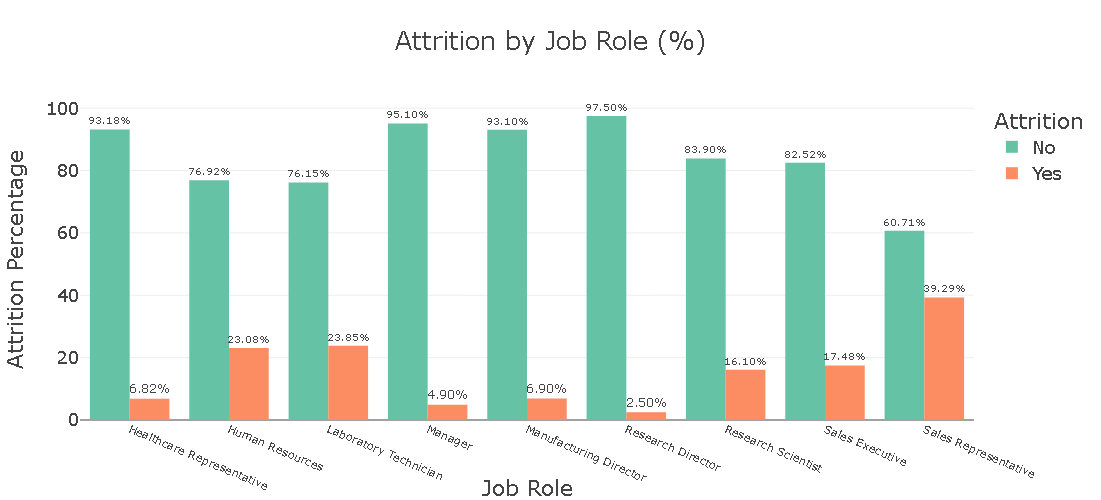
\includegraphics[keepaspectratio]{HR_Analytics_files/figure-pdf/cell-72-output-1.png}}

\subsection{Visualizing Attrition by Age
Group}\label{visualizing-attrition-by-age-group}

This chart helps analyze how attrition varies across different age
groups, providing insight into which age ranges may be more prone to
leaving the company. Grouping: We group the data by AgeGroup and
Attrition to calculate the number of employees who left or stayed in
each age range.

Percentage Calculation: For each AgeGroup, we calculate the percentage
of employees who left (Attrition = Yes).

Visualization: A grouped bar chart shows attrition percentages by age
group with distinct colors for each attrition category.

Styling: The layout is customized for clear labels and a professional
presentation using a light and clean color theme.

Exporting: The chart is saved in JPG, PNG, and HTML formats for easy use
in presentations and dashboards.

This chart is valuable for understanding if younger or older employees
are more likely to leave, helping inform age-specific retention
strategies.

\begin{Shaded}
\begin{Highlighting}[]
\NormalTok{attrition\_by\_age }\OperatorTok{=}\NormalTok{ HR\_Analytics\_df.groupby([}\StringTok{\textquotesingle{}AgeGroup\textquotesingle{}}\NormalTok{, }\StringTok{\textquotesingle{}Attrition\textquotesingle{}}\NormalTok{]).size().reset\_index(name}\OperatorTok{=}\StringTok{\textquotesingle{}count\textquotesingle{}}\NormalTok{)}
\NormalTok{total\_per\_age }\OperatorTok{=}\NormalTok{ attrition\_by\_age.groupby(}\StringTok{\textquotesingle{}AgeGroup\textquotesingle{}}\NormalTok{)[}\StringTok{\textquotesingle{}count\textquotesingle{}}\NormalTok{].transform(}\StringTok{\textquotesingle{}sum\textquotesingle{}}\NormalTok{)}
\NormalTok{attrition\_by\_age[}\StringTok{\textquotesingle{}percentage\textquotesingle{}}\NormalTok{] }\OperatorTok{=} \BuiltInTok{round}\NormalTok{((attrition\_by\_age[}\StringTok{\textquotesingle{}count\textquotesingle{}}\NormalTok{] }\OperatorTok{/}\NormalTok{ total\_per\_age) }\OperatorTok{*} \DecValTok{100}\NormalTok{, }\DecValTok{2}\NormalTok{)}

\NormalTok{fig }\OperatorTok{=}\NormalTok{ px.bar(attrition\_by\_age,}
\NormalTok{             x}\OperatorTok{=}\StringTok{\textquotesingle{}AgeGroup\textquotesingle{}}\NormalTok{,}
\NormalTok{             y}\OperatorTok{=}\StringTok{\textquotesingle{}percentage\textquotesingle{}}\NormalTok{,}
\NormalTok{             color}\OperatorTok{=}\StringTok{\textquotesingle{}Attrition\textquotesingle{}}\NormalTok{,}
\NormalTok{             title}\OperatorTok{=}\StringTok{\textquotesingle{}Attrition by Age Group (\%)\textquotesingle{}}\NormalTok{,}
\NormalTok{             color\_discrete\_sequence}\OperatorTok{=}\NormalTok{[}\StringTok{"\#4dd0e1"}\NormalTok{, }\StringTok{"\#00695c"}\NormalTok{],}
\NormalTok{             barmode}\OperatorTok{=}\StringTok{\textquotesingle{}group\textquotesingle{}}\NormalTok{,}
\NormalTok{             text}\OperatorTok{=}\StringTok{\textquotesingle{}percentage\textquotesingle{}}\NormalTok{,}
\NormalTok{             width}\OperatorTok{=}\DecValTok{700}\NormalTok{,}
\NormalTok{             height}\OperatorTok{=}\DecValTok{500}\NormalTok{)}

\NormalTok{fig.update\_layout(template}\OperatorTok{=}\StringTok{"presentation"}\NormalTok{,}
\NormalTok{                  xaxis\_title}\OperatorTok{=}\StringTok{\textquotesingle{}Age Group\textquotesingle{}}\NormalTok{,}
\NormalTok{                  yaxis\_title}\OperatorTok{=}\StringTok{\textquotesingle{}Attrition Percentage\textquotesingle{}}\NormalTok{,}
\NormalTok{                  legend\_title}\OperatorTok{=}\BuiltInTok{dict}\NormalTok{(text}\OperatorTok{=}\StringTok{\textquotesingle{}Attrition\textquotesingle{}}\NormalTok{),}
\NormalTok{                  paper\_bgcolor}\OperatorTok{=}\StringTok{"rgba(0,0,0,0)"}\NormalTok{,}
\NormalTok{                  plot\_bgcolor}\OperatorTok{=}\StringTok{"rgba(0,0,0,0)"}\NormalTok{)}

\NormalTok{fig.update\_traces(texttemplate}\OperatorTok{=}\StringTok{\textquotesingle{}\%}\SpecialCharTok{\{text:.2f\}}\StringTok{\%\textquotesingle{}}\NormalTok{, textposition}\OperatorTok{=}\StringTok{\textquotesingle{}outside\textquotesingle{}}\NormalTok{)}
\NormalTok{fig.show()}

\NormalTok{fig.write\_image(os.path.join(results\_dir, }\StringTok{\textquotesingle{}attrition\_by\_age.jpg\textquotesingle{}}\NormalTok{))}
\NormalTok{fig.write\_image(os.path.join(results\_dir, }\StringTok{\textquotesingle{}attrition\_by\_age.png\textquotesingle{}}\NormalTok{))}
\NormalTok{fig.write\_html(os.path.join(results\_dir, }\StringTok{\textquotesingle{}attrition\_by\_age.html\textquotesingle{}}\NormalTok{))}
\end{Highlighting}
\end{Shaded}

\pandocbounded{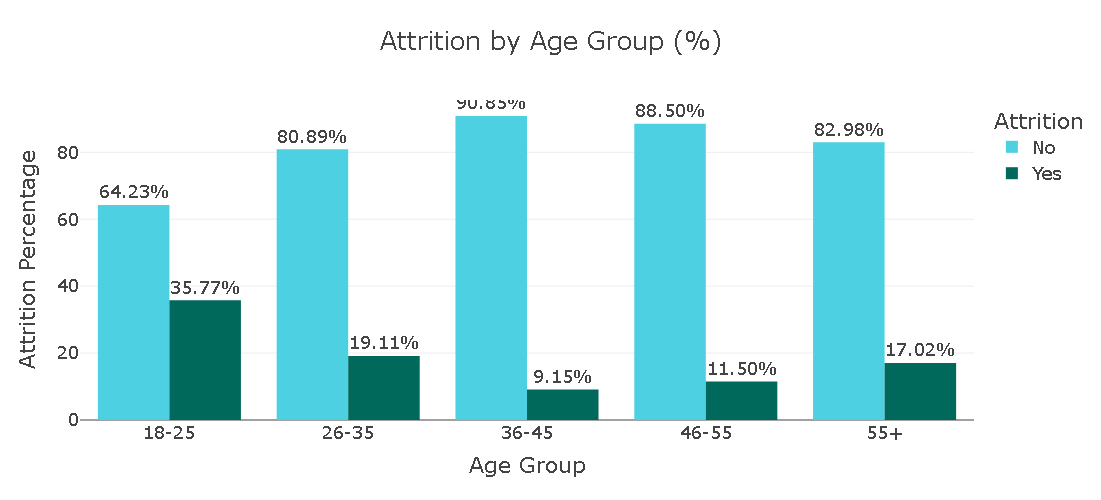
\includegraphics[keepaspectratio]{HR_Analytics_files/figure-pdf/cell-73-output-1.png}}

\subsection{Visualizing Attrition by Overtime
Status}\label{visualizing-attrition-by-overtime-status}

This analysis shows how employee attrition differs between those who
work overtime and those who don't, highlighting the impact of overtime
on turnover. Grouping: We group employees by OverTime status and
Attrition to count how many left or stayed in each group.

Percentage Calculation: For each overtime category, we calculate the
percentage of employees who left.

Visualization: The grouped bar chart compares attrition rates between
employees working overtime versus those who do not.

Styling: The chart uses custom colors and a clean layout for better
readability.

Exporting: Saved as JPG, PNG, and HTML files to support sharing and
embedding in reports.

This insight helps understand whether overtime work correlates with
higher employee attrition.

\begin{Shaded}
\begin{Highlighting}[]
\NormalTok{overtime\_attrition }\OperatorTok{=}\NormalTok{ HR\_Analytics\_df.groupby([}\StringTok{\textquotesingle{}OverTime\textquotesingle{}}\NormalTok{, }\StringTok{\textquotesingle{}Attrition\textquotesingle{}}\NormalTok{]).size().reset\_index(name}\OperatorTok{=}\StringTok{\textquotesingle{}count\textquotesingle{}}\NormalTok{)}
\NormalTok{total\_per\_ot }\OperatorTok{=}\NormalTok{ overtime\_attrition.groupby(}\StringTok{\textquotesingle{}OverTime\textquotesingle{}}\NormalTok{)[}\StringTok{\textquotesingle{}count\textquotesingle{}}\NormalTok{].transform(}\StringTok{\textquotesingle{}sum\textquotesingle{}}\NormalTok{)}
\NormalTok{overtime\_attrition[}\StringTok{\textquotesingle{}percentage\textquotesingle{}}\NormalTok{] }\OperatorTok{=} \BuiltInTok{round}\NormalTok{((overtime\_attrition[}\StringTok{\textquotesingle{}count\textquotesingle{}}\NormalTok{] }\OperatorTok{/}\NormalTok{ total\_per\_ot) }\OperatorTok{*} \DecValTok{100}\NormalTok{, }\DecValTok{2}\NormalTok{)}

\NormalTok{fig }\OperatorTok{=}\NormalTok{ px.bar(overtime\_attrition,}
\NormalTok{             x}\OperatorTok{=}\StringTok{\textquotesingle{}OverTime\textquotesingle{}}\NormalTok{,}
\NormalTok{             y}\OperatorTok{=}\StringTok{\textquotesingle{}percentage\textquotesingle{}}\NormalTok{,}
\NormalTok{             color}\OperatorTok{=}\StringTok{\textquotesingle{}Attrition\textquotesingle{}}\NormalTok{,}
\NormalTok{             title}\OperatorTok{=}\StringTok{\textquotesingle{}Attrition by Overtime (\%)\textquotesingle{}}\NormalTok{,}
\NormalTok{             color\_discrete\_sequence}\OperatorTok{=}\NormalTok{[}\StringTok{"\#26c6da"}\NormalTok{, }\StringTok{"\#004d40"}\NormalTok{],}
\NormalTok{             barmode}\OperatorTok{=}\StringTok{\textquotesingle{}group\textquotesingle{}}\NormalTok{,}
\NormalTok{             text}\OperatorTok{=}\StringTok{\textquotesingle{}percentage\textquotesingle{}}\NormalTok{,}
\NormalTok{             width}\OperatorTok{=}\DecValTok{400}\NormalTok{,}
\NormalTok{             height}\OperatorTok{=}\DecValTok{500}\NormalTok{)}

\NormalTok{fig.update\_layout(template}\OperatorTok{=}\StringTok{"presentation"}\NormalTok{,}
\NormalTok{                  xaxis\_title}\OperatorTok{=}\StringTok{\textquotesingle{}OverTime\textquotesingle{}}\NormalTok{,}
\NormalTok{                  yaxis\_title}\OperatorTok{=}\StringTok{\textquotesingle{}Attrition Percentage\textquotesingle{}}\NormalTok{,}
\NormalTok{                  legend\_title}\OperatorTok{=}\BuiltInTok{dict}\NormalTok{(text}\OperatorTok{=}\StringTok{\textquotesingle{}Attrition\textquotesingle{}}\NormalTok{),}
\NormalTok{                  paper\_bgcolor}\OperatorTok{=}\StringTok{"rgba(0,0,0,0)"}\NormalTok{,}
\NormalTok{                  plot\_bgcolor}\OperatorTok{=}\StringTok{"rgba(0,0,0,0)"}\NormalTok{)}

\NormalTok{fig.update\_traces(texttemplate}\OperatorTok{=}\StringTok{\textquotesingle{}\%}\SpecialCharTok{\{text:.2f\}}\StringTok{\%\textquotesingle{}}\NormalTok{, textposition}\OperatorTok{=}\StringTok{\textquotesingle{}outside\textquotesingle{}}\NormalTok{)}
\NormalTok{fig.show()}

\NormalTok{fig.write\_image(os.path.join(results\_dir, }\StringTok{\textquotesingle{}attrition\_by\_overtime.jpg\textquotesingle{}}\NormalTok{))}
\NormalTok{fig.write\_image(os.path.join(results\_dir, }\StringTok{\textquotesingle{}attrition\_by\_overtime.png\textquotesingle{}}\NormalTok{))}
\NormalTok{fig.write\_html(os.path.join(results\_dir, }\StringTok{\textquotesingle{}attrition\_by\_overtime.html\textquotesingle{}}\NormalTok{))}
\end{Highlighting}
\end{Shaded}

\pandocbounded{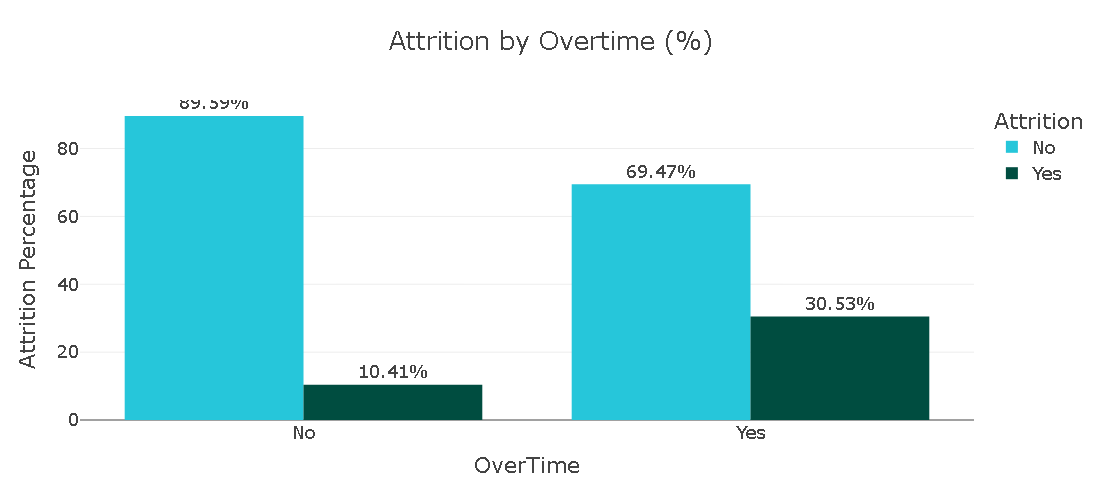
\includegraphics[keepaspectratio]{HR_Analytics_files/figure-pdf/cell-74-output-1.png}}

\subsection{Visualizing Gender Distribution in the
Company}\label{visualizing-gender-distribution-in-the-company}

This chart shows the percentage breakdown of employees by gender,
providing insight into workforce diversity. Calculation: We calculate
the normalized counts (percentages) of each gender in the dataset.

Visualization: A pastel-colored bar chart displays the percentage of
male and female employees.

Layout: The chart is styled for clarity, with percentage labels shown
outside the bars and no legend (since colors correspond directly to
gender labels).

Exporting: Saved as JPG, PNG, and HTML for easy sharing and embedding.

This visualization provides a quick understanding of gender
representation within the company.

\begin{Shaded}
\begin{Highlighting}[]
\NormalTok{gender\_dist }\OperatorTok{=}\NormalTok{ HR\_Analytics\_df[}\StringTok{\textquotesingle{}Gender\textquotesingle{}}\NormalTok{].value\_counts(normalize}\OperatorTok{=}\VariableTok{True}\NormalTok{).reset\_index()}
\NormalTok{gender\_dist.columns }\OperatorTok{=}\NormalTok{ [}\StringTok{\textquotesingle{}Gender\textquotesingle{}}\NormalTok{, }\StringTok{\textquotesingle{}Percentage\textquotesingle{}}\NormalTok{]}
\NormalTok{gender\_dist[}\StringTok{\textquotesingle{}Percentage\textquotesingle{}}\NormalTok{] }\OperatorTok{*=} \DecValTok{100}

\NormalTok{fig }\OperatorTok{=}\NormalTok{ px.bar(}
\NormalTok{    gender\_dist,}
\NormalTok{    x}\OperatorTok{=}\StringTok{\textquotesingle{}Gender\textquotesingle{}}\NormalTok{,}
\NormalTok{    y}\OperatorTok{=}\StringTok{\textquotesingle{}Percentage\textquotesingle{}}\NormalTok{,}
\NormalTok{    text}\OperatorTok{=}\StringTok{\textquotesingle{}Percentage\textquotesingle{}}\NormalTok{,}
\NormalTok{    color}\OperatorTok{=}\StringTok{\textquotesingle{}Gender\textquotesingle{}}\NormalTok{,}
\NormalTok{    color\_discrete\_sequence}\OperatorTok{=}\NormalTok{px.colors.qualitative.Pastel1,}
\NormalTok{    title}\OperatorTok{=}\StringTok{\textquotesingle{}Gender Distribution (\%)\textquotesingle{}}\NormalTok{,}
\NormalTok{    width}\OperatorTok{=}\DecValTok{400}\NormalTok{,     }
\NormalTok{    height}\OperatorTok{=}\DecValTok{700}    
\NormalTok{)}

\NormalTok{fig.update\_layout(}
\NormalTok{    template}\OperatorTok{=}\StringTok{"presentation"}\NormalTok{,}
\NormalTok{    xaxis\_title}\OperatorTok{=}\StringTok{\textquotesingle{}Gender\textquotesingle{}}\NormalTok{,}
\NormalTok{    yaxis\_title}\OperatorTok{=}\StringTok{\textquotesingle{}Percentage of Employees\textquotesingle{}}\NormalTok{,}
\NormalTok{    showlegend}\OperatorTok{=}\VariableTok{False}\NormalTok{,}
\NormalTok{    paper\_bgcolor}\OperatorTok{=}\StringTok{"rgba(0,0,0,0)"}\NormalTok{,}
\NormalTok{    plot\_bgcolor}\OperatorTok{=}\StringTok{"rgba(0,0,0,0)"}
\NormalTok{)}

\NormalTok{fig.update\_traces(texttemplate}\OperatorTok{=}\StringTok{\textquotesingle{}\%}\SpecialCharTok{\{text:.2f\}}\StringTok{\%\textquotesingle{}}\NormalTok{, textposition}\OperatorTok{=}\StringTok{\textquotesingle{}outside\textquotesingle{}}\NormalTok{)}
\NormalTok{fig.show()}

\NormalTok{fig.write\_image(os.path.join(results\_dir, }\StringTok{\textquotesingle{}gender\_distribution.jpg\textquotesingle{}}\NormalTok{))}
\NormalTok{fig.write\_image(os.path.join(results\_dir, }\StringTok{\textquotesingle{}gender\_distribution.png\textquotesingle{}}\NormalTok{))}
\NormalTok{fig.write\_html(os.path.join(results\_dir, }\StringTok{\textquotesingle{}gender\_distribution.html\textquotesingle{}}\NormalTok{))}
\end{Highlighting}
\end{Shaded}

\pandocbounded{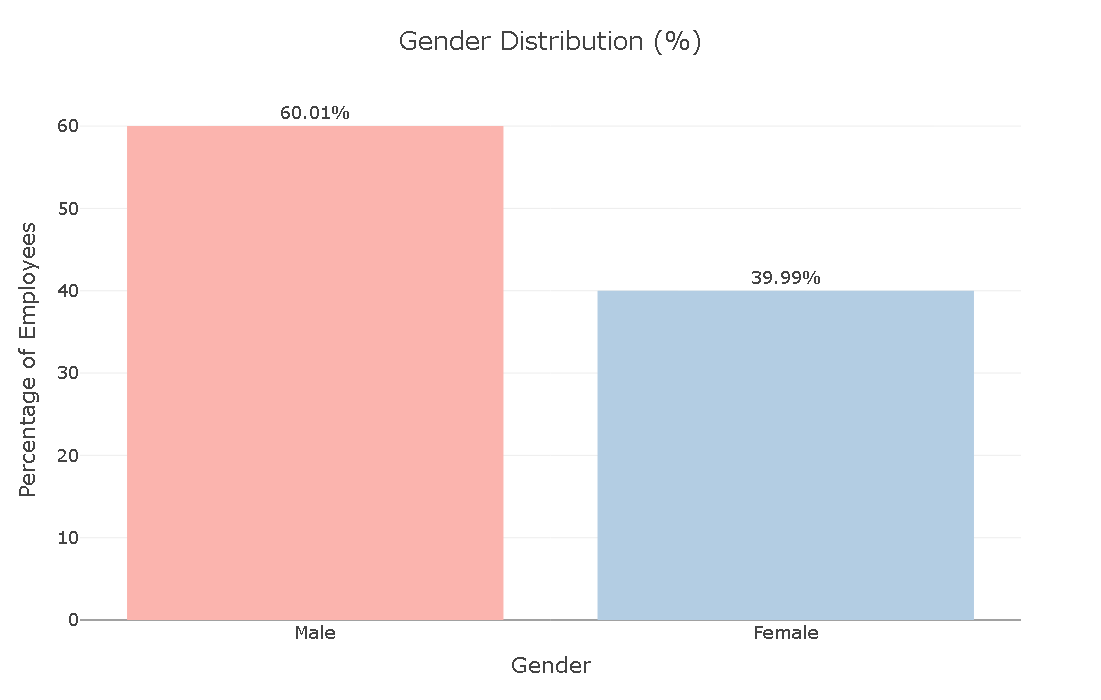
\includegraphics[keepaspectratio]{HR_Analytics_files/figure-pdf/cell-75-output-1.png}}

\subsection{Visualizing Job Satisfaction
Levels}\label{visualizing-job-satisfaction-levels}

This chart illustrates the distribution of employee job satisfaction
ratings, helping to understand overall workplace morale. Calculation: We
compute the percentage of employees for each job satisfaction level
(from 1 to 4).

Visualization: A sequential blue color scale bar chart represents the
satisfaction levels.

Layout: The chart is styled cleanly, with percentage labels on top of
the bars and no legend since colors directly map to satisfaction levels.

Exporting: The visualization is saved in JPG, PNG, and HTML formats for
easy sharing and embedding.

This chart helps identify how satisfied employees are with their jobs
overall.

\begin{Shaded}
\begin{Highlighting}[]
\NormalTok{job\_satisfaction }\OperatorTok{=}\NormalTok{ HR\_Analytics\_df[}\StringTok{\textquotesingle{}JobSatisfaction\textquotesingle{}}\NormalTok{].value\_counts(normalize}\OperatorTok{=}\VariableTok{True}\NormalTok{).sort\_index().reset\_index()}
\NormalTok{job\_satisfaction.columns }\OperatorTok{=}\NormalTok{ [}\StringTok{\textquotesingle{}Satisfaction Level\textquotesingle{}}\NormalTok{, }\StringTok{\textquotesingle{}Percentage\textquotesingle{}}\NormalTok{]}
\NormalTok{job\_satisfaction[}\StringTok{\textquotesingle{}Percentage\textquotesingle{}}\NormalTok{] }\OperatorTok{*=} \DecValTok{100}

\NormalTok{fig }\OperatorTok{=}\NormalTok{ px.bar(job\_satisfaction,}
\NormalTok{             x}\OperatorTok{=}\StringTok{\textquotesingle{}Satisfaction Level\textquotesingle{}}\NormalTok{,}
\NormalTok{             y}\OperatorTok{=}\StringTok{\textquotesingle{}Percentage\textquotesingle{}}\NormalTok{,}
\NormalTok{             text}\OperatorTok{=}\StringTok{\textquotesingle{}Percentage\textquotesingle{}}\NormalTok{,}
\NormalTok{             color}\OperatorTok{=}\StringTok{\textquotesingle{}Satisfaction Level\textquotesingle{}}\NormalTok{,}
\NormalTok{             color\_discrete\_sequence}\OperatorTok{=}\NormalTok{px.colors.sequential.Blues,}
\NormalTok{             title}\OperatorTok{=}\StringTok{\textquotesingle{}Job Satisfaction Levels (\%)\textquotesingle{}}\NormalTok{,}
\NormalTok{             width}\OperatorTok{=}\DecValTok{400}\NormalTok{,}
\NormalTok{             height}\OperatorTok{=}\DecValTok{400}\NormalTok{)}

\NormalTok{fig.update\_layout(template}\OperatorTok{=}\StringTok{"presentation"}\NormalTok{,}
\NormalTok{                  xaxis\_title}\OperatorTok{=}\StringTok{\textquotesingle{}Satisfaction Level (1–4)\textquotesingle{}}\NormalTok{,}
\NormalTok{                  yaxis\_title}\OperatorTok{=}\StringTok{\textquotesingle{}Percentage of Employees\textquotesingle{}}\NormalTok{,}
\NormalTok{                  width}\OperatorTok{=}\DecValTok{700}\NormalTok{,}
\NormalTok{                  height}\OperatorTok{=}\DecValTok{600}\NormalTok{,}
\NormalTok{                  showlegend}\OperatorTok{=}\VariableTok{False}\NormalTok{,}
\NormalTok{                  paper\_bgcolor}\OperatorTok{=}\StringTok{"rgba(0,0,0,0)"}\NormalTok{,}
\NormalTok{                  plot\_bgcolor}\OperatorTok{=}\StringTok{"rgba(0,0,0,0)"}\NormalTok{)}


\NormalTok{fig.update\_traces(texttemplate}\OperatorTok{=}\StringTok{\textquotesingle{}\%}\SpecialCharTok{\{text:.2f\}}\StringTok{\%\textquotesingle{}}\NormalTok{, textposition}\OperatorTok{=}\StringTok{\textquotesingle{}outside\textquotesingle{}}\NormalTok{)}
\NormalTok{fig.show()}

\NormalTok{fig.write\_image(os.path.join(results\_dir, }\StringTok{\textquotesingle{}job\_satisfaction.jpg\textquotesingle{}}\NormalTok{))}
\NormalTok{fig.write\_image(os.path.join(results\_dir, }\StringTok{\textquotesingle{}job\_satisfaction.png\textquotesingle{}}\NormalTok{))}
\NormalTok{fig.write\_html(os.path.join(results\_dir, }\StringTok{\textquotesingle{}job\_satisfaction.html\textquotesingle{}}\NormalTok{))}
\end{Highlighting}
\end{Shaded}

\pandocbounded{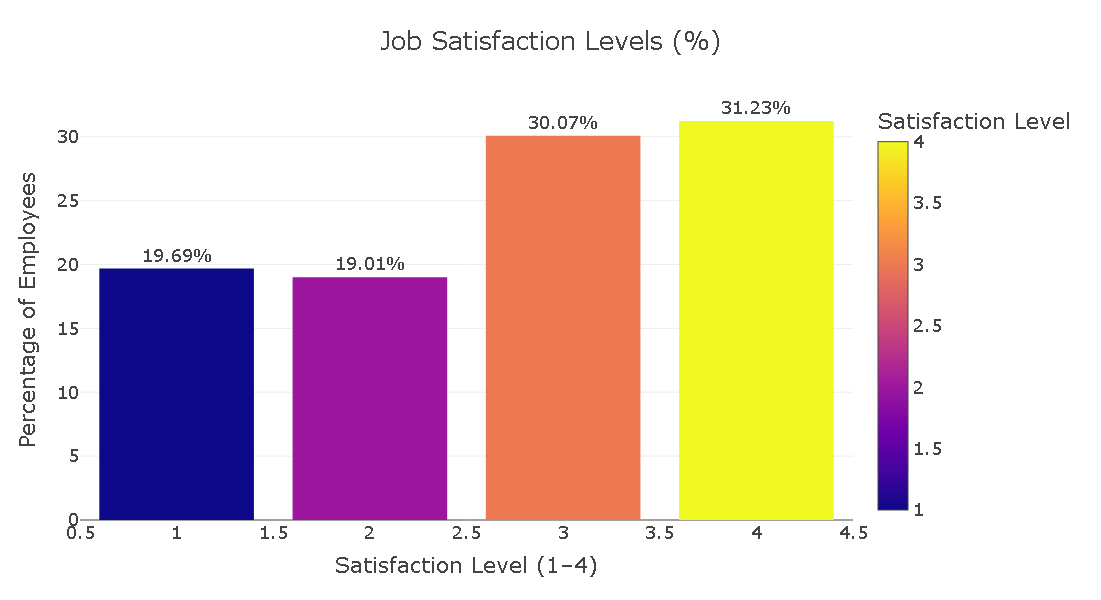
\includegraphics[keepaspectratio]{HR_Analytics_files/figure-pdf/cell-76-output-1.png}}

\subsection{Visualizing Average Monthly Income by Job
Level}\label{visualizing-average-monthly-income-by-job-level}

This chart displays the average monthly income of employees across
different job levels, highlighting pay disparities within the company.
Calculation: We compute the mean monthly income for each job level.

Visualization: A bar chart with color-coded job levels shows average
income, with values labeled above each bar.

Layout: Clean design with no legend, as job levels are self-explanatory
on the x-axis.

Exporting: Saved as JPG, PNG, and HTML for use in reports or dashboards.

This chart helps understand how compensation scales with job level in
the organization

\begin{Shaded}
\begin{Highlighting}[]
\NormalTok{income\_by\_level }\OperatorTok{=}\NormalTok{ HR\_Analytics\_df.groupby(}\StringTok{\textquotesingle{}JobLevel\textquotesingle{}}\NormalTok{)[}\StringTok{\textquotesingle{}MonthlyIncome\textquotesingle{}}\NormalTok{].mean().reset\_index()}

\NormalTok{fig }\OperatorTok{=}\NormalTok{ px.bar(income\_by\_level,}
\NormalTok{             x}\OperatorTok{=}\StringTok{\textquotesingle{}JobLevel\textquotesingle{}}\NormalTok{,}
\NormalTok{             y}\OperatorTok{=}\StringTok{\textquotesingle{}MonthlyIncome\textquotesingle{}}\NormalTok{,}
\NormalTok{             text}\OperatorTok{=}\StringTok{\textquotesingle{}MonthlyIncome\textquotesingle{}}\NormalTok{,}
\NormalTok{             title}\OperatorTok{=}\StringTok{\textquotesingle{}Average Monthly Income by Job Level\textquotesingle{}}\NormalTok{,}
\NormalTok{             color}\OperatorTok{=}\StringTok{\textquotesingle{}JobLevel\textquotesingle{}}\NormalTok{,}
\NormalTok{             color\_discrete\_sequence}\OperatorTok{=}\NormalTok{[}\StringTok{\textquotesingle{}red\textquotesingle{}}\NormalTok{, }\StringTok{\textquotesingle{}green\textquotesingle{}}\NormalTok{],}
\NormalTok{             width}\OperatorTok{=}\DecValTok{600}\NormalTok{,}
\NormalTok{             height}\OperatorTok{=}\DecValTok{700}\NormalTok{)}

\NormalTok{fig.update\_layout(template}\OperatorTok{=}\StringTok{"presentation"}\NormalTok{,}
\NormalTok{                  xaxis\_title}\OperatorTok{=}\StringTok{\textquotesingle{}Job Level\textquotesingle{}}\NormalTok{,}
\NormalTok{                  yaxis\_title}\OperatorTok{=}\StringTok{\textquotesingle{}Average Monthly Income\textquotesingle{}}\NormalTok{,}
\NormalTok{                  showlegend}\OperatorTok{=}\VariableTok{False}\NormalTok{,}
\NormalTok{                  paper\_bgcolor}\OperatorTok{=}\StringTok{"rgba(0,0,0,0)"}\NormalTok{,}
\NormalTok{                  plot\_bgcolor}\OperatorTok{=}\StringTok{"rgba(0,0,0,0)"}\NormalTok{)}

\NormalTok{fig.update\_traces(texttemplate}\OperatorTok{=}\StringTok{\textquotesingle{}\%}\SpecialCharTok{\{text:.0f\}}\StringTok{\textquotesingle{}}\NormalTok{, textposition}\OperatorTok{=}\StringTok{\textquotesingle{}outside\textquotesingle{}}\NormalTok{)}
\NormalTok{fig.show()}

\NormalTok{fig.write\_image(os.path.join(results\_dir, }\StringTok{\textquotesingle{}income\_by\_joblevel.jpg\textquotesingle{}}\NormalTok{))}
\NormalTok{fig.write\_image(os.path.join(results\_dir, }\StringTok{\textquotesingle{}income\_by\_joblevel.png\textquotesingle{}}\NormalTok{))}
\NormalTok{fig.write\_html(os.path.join(results\_dir, }\StringTok{\textquotesingle{}income\_by\_joblevel.html\textquotesingle{}}\NormalTok{))}
\end{Highlighting}
\end{Shaded}

\pandocbounded{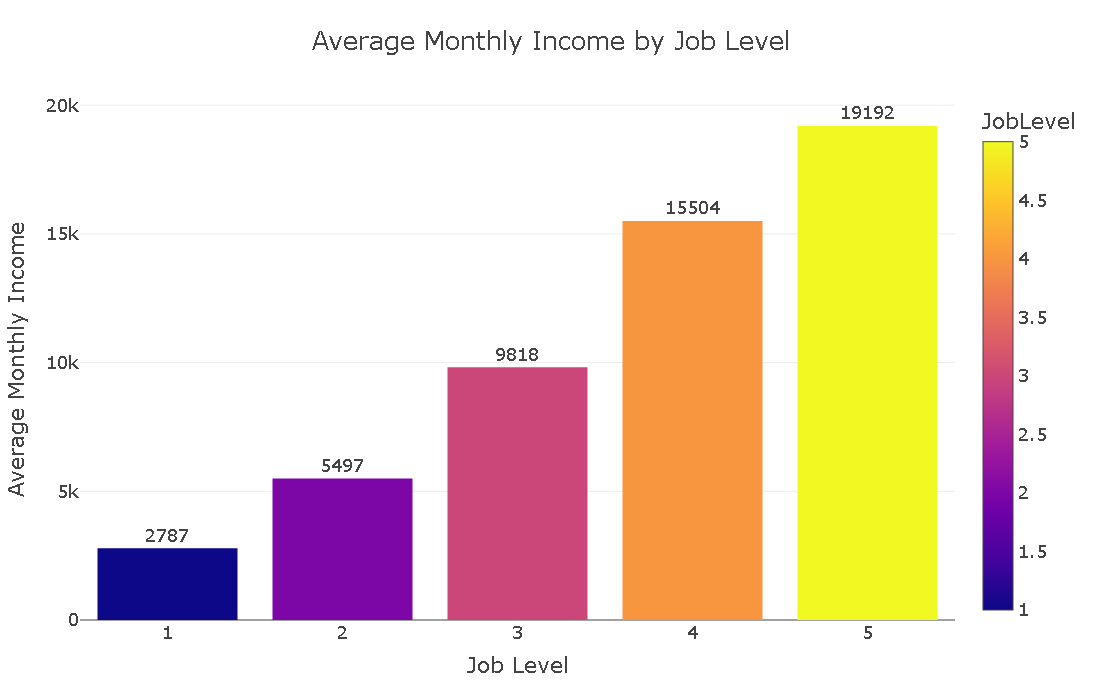
\includegraphics[keepaspectratio]{HR_Analytics_files/figure-pdf/cell-77-output-1.png}}

\subsection{Distribution of Job Levels by Education
Field}\label{distribution-of-job-levels-by-education-field}

This stacked bar chart shows how employees are distributed across
different job levels within each education field, highlighting the
relationship between education background and job hierarchy. Grouping:
Counts employees by their education field and job level.

Visualization: A stacked bar chart reveals how job levels stack within
each education field.

Styling: Angled x-axis labels improve readability; color-coded job
levels aid interpretation.

Exporting: Saved as JPG, PNG, and HTML for easy integration in reports
and presentations.

This visualization helps identify education backgrounds that correlate
with higher or lower job levels.

\begin{Shaded}
\begin{Highlighting}[]
\NormalTok{edu\_job }\OperatorTok{=}\NormalTok{ HR\_Analytics\_df.groupby([}\StringTok{\textquotesingle{}EducationField\textquotesingle{}}\NormalTok{, }\StringTok{\textquotesingle{}JobLevel\textquotesingle{}}\NormalTok{]).size().reset\_index(name}\OperatorTok{=}\StringTok{\textquotesingle{}count\textquotesingle{}}\NormalTok{)}

\NormalTok{fig }\OperatorTok{=}\NormalTok{ px.bar(}
\NormalTok{    edu\_job,}
\NormalTok{    x}\OperatorTok{=}\StringTok{\textquotesingle{}EducationField\textquotesingle{}}\NormalTok{,}
\NormalTok{    y}\OperatorTok{=}\StringTok{\textquotesingle{}count\textquotesingle{}}\NormalTok{,}
\NormalTok{    color}\OperatorTok{=}\StringTok{\textquotesingle{}JobLevel\textquotesingle{}}\NormalTok{,}
\NormalTok{    title}\OperatorTok{=}\StringTok{\textquotesingle{}Distribution of Job Levels by Education Field\textquotesingle{}}\NormalTok{,}
\NormalTok{    barmode}\OperatorTok{=}\StringTok{\textquotesingle{}stack\textquotesingle{}}\NormalTok{,}
\NormalTok{    text}\OperatorTok{=}\StringTok{\textquotesingle{}count\textquotesingle{}}\NormalTok{,}
\NormalTok{    color\_discrete\_sequence}\OperatorTok{=}\NormalTok{px.colors.qualitative.Set2,  }
\NormalTok{    width}\OperatorTok{=}\DecValTok{900}\NormalTok{,     }
\NormalTok{    height}\OperatorTok{=}\DecValTok{600}     
\NormalTok{)}

\NormalTok{fig.update\_layout(}
\NormalTok{    template}\OperatorTok{=}\StringTok{\textquotesingle{}presentation\textquotesingle{}}\NormalTok{,}
\NormalTok{    xaxis\_title}\OperatorTok{=}\StringTok{\textquotesingle{}Education Field\textquotesingle{}}\NormalTok{,}
\NormalTok{    yaxis\_title}\OperatorTok{=}\StringTok{\textquotesingle{}Number of Employees\textquotesingle{}}\NormalTok{,}
\NormalTok{    xaxis\_tickangle}\OperatorTok{=}\DecValTok{60}\NormalTok{,             }
\NormalTok{    xaxis\_tickfont}\OperatorTok{=}\BuiltInTok{dict}\NormalTok{(size}\OperatorTok{=}\DecValTok{11}\NormalTok{),   }
\NormalTok{    legend\_title}\OperatorTok{=}\BuiltInTok{dict}\NormalTok{(text}\OperatorTok{=}\StringTok{\textquotesingle{}Job Level\textquotesingle{}}\NormalTok{),}
\NormalTok{    paper\_bgcolor}\OperatorTok{=}\StringTok{"rgba(0,0,0,0)"}\NormalTok{,}
\NormalTok{    plot\_bgcolor}\OperatorTok{=}\StringTok{"rgba(0,0,0,0)"}
\NormalTok{)}

\NormalTok{fig.update\_traces(texttemplate}\OperatorTok{=}\StringTok{\textquotesingle{}\%}\SpecialCharTok{\{text\}}\StringTok{\textquotesingle{}}\NormalTok{, textposition}\OperatorTok{=}\StringTok{\textquotesingle{}inside\textquotesingle{}}\NormalTok{)}

\NormalTok{fig.show()}

\CommentTok{\# Save visuals}
\NormalTok{fig.write\_image(os.path.join(results\_dir, }\StringTok{\textquotesingle{}Joblevel\_edufield.jpg\textquotesingle{}}\NormalTok{))}
\NormalTok{fig.write\_image(os.path.join(results\_dir, }\StringTok{\textquotesingle{}Joblevel\_edufield.png\textquotesingle{}}\NormalTok{))}
\NormalTok{fig.write\_html(os.path.join(results\_dir, }\StringTok{\textquotesingle{}Joblevel\_edufield.html\textquotesingle{}}\NormalTok{))}
\end{Highlighting}
\end{Shaded}

\pandocbounded{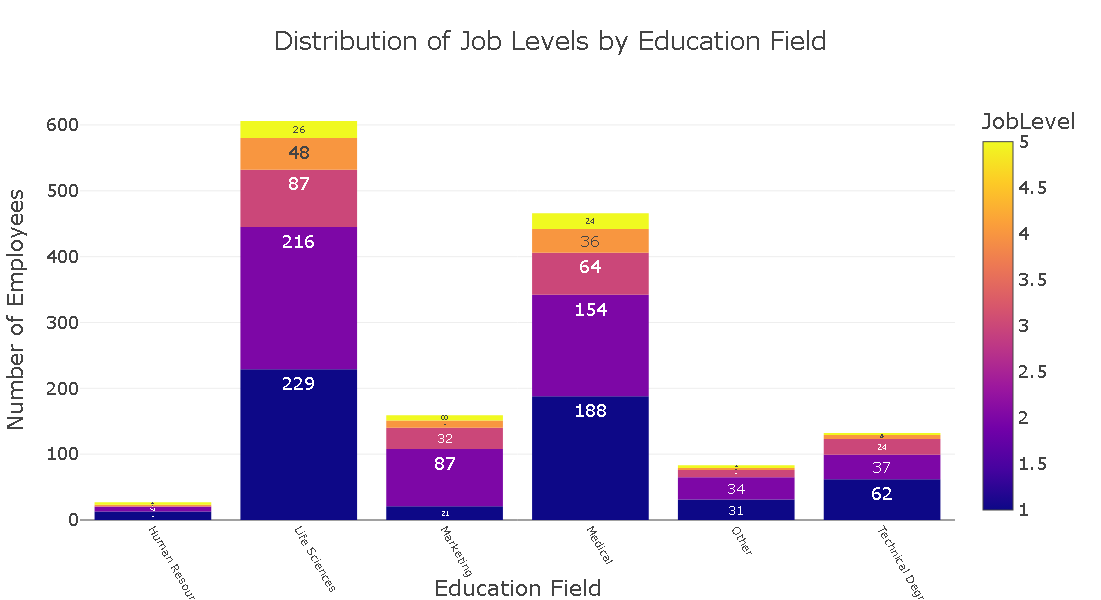
\includegraphics[keepaspectratio]{HR_Analytics_files/figure-pdf/cell-78-output-1.png}}

\subsection{Years Since Last Promotion by Job
Role}\label{years-since-last-promotion-by-job-role}

This stacked bar chart displays the distribution of employees across job
roles based on the number of years since their last promotion, providing
insight into promotion patterns by role. Grouping: Aggregates employee
counts by their job role and years since last promotion.

Visualization: Stacked bars show how many employees in each role have
different promotion intervals.

Styling: Angled x-axis labels improve readability; distinct colors
represent different promotion year groups.

Exporting: Saved as JPG, PNG, and HTML files for reporting and
presentation.

This chart helps HR identify roles with recent or delayed promotions,
supporting career development planning.

\begin{Shaded}
\begin{Highlighting}[]
\NormalTok{promo\_by\_role }\OperatorTok{=}\NormalTok{ HR\_Analytics\_df.groupby([}\StringTok{\textquotesingle{}JobRole\textquotesingle{}}\NormalTok{, }\StringTok{\textquotesingle{}YearsSinceLastPromotion\textquotesingle{}}\NormalTok{]).size().reset\_index(name}\OperatorTok{=}\StringTok{\textquotesingle{}count\textquotesingle{}}\NormalTok{)}

\NormalTok{fig }\OperatorTok{=}\NormalTok{ px.bar(}
\NormalTok{    promo\_by\_role,}
\NormalTok{    x}\OperatorTok{=}\StringTok{\textquotesingle{}JobRole\textquotesingle{}}\NormalTok{,}
\NormalTok{    y}\OperatorTok{=}\StringTok{\textquotesingle{}count\textquotesingle{}}\NormalTok{,}
\NormalTok{    color}\OperatorTok{=}\StringTok{\textquotesingle{}YearsSinceLastPromotion\textquotesingle{}}\NormalTok{,}
\NormalTok{    title}\OperatorTok{=}\StringTok{\textquotesingle{}Years Since Last Promotion by Job Role\textquotesingle{}}\NormalTok{,}
\NormalTok{    barmode}\OperatorTok{=}\StringTok{\textquotesingle{}stack\textquotesingle{}}\NormalTok{,}
\NormalTok{    text}\OperatorTok{=}\StringTok{\textquotesingle{}count\textquotesingle{}}\NormalTok{,}
\NormalTok{    color\_discrete\_sequence}\OperatorTok{=}\NormalTok{px.colors.qualitative.Set3,}
\NormalTok{    width}\OperatorTok{=}\DecValTok{900}\NormalTok{,   }
\NormalTok{    height}\OperatorTok{=}\DecValTok{1000}  
\NormalTok{)}

\NormalTok{fig.update\_layout(}
\NormalTok{    template}\OperatorTok{=}\StringTok{\textquotesingle{}presentation\textquotesingle{}}\NormalTok{,}
\NormalTok{    xaxis\_title}\OperatorTok{=}\StringTok{\textquotesingle{}\textquotesingle{}}\NormalTok{,  }
\NormalTok{    yaxis\_title}\OperatorTok{=}\StringTok{\textquotesingle{}Employee Count\textquotesingle{}}\NormalTok{,}
\NormalTok{    xaxis\_tickangle}\OperatorTok{=}\DecValTok{20}\NormalTok{,           }
\NormalTok{    xaxis\_tickfont}\OperatorTok{=}\BuiltInTok{dict}\NormalTok{(size}\OperatorTok{=}\DecValTok{11}\NormalTok{), }
\NormalTok{    legend\_title}\OperatorTok{=}\BuiltInTok{dict}\NormalTok{(text}\OperatorTok{=}\StringTok{\textquotesingle{}Years Since Last Promotion\textquotesingle{}}\NormalTok{),}
\NormalTok{    paper\_bgcolor}\OperatorTok{=}\StringTok{"rgba(0,0,0,0)"}\NormalTok{,}
\NormalTok{    plot\_bgcolor}\OperatorTok{=}\StringTok{"rgba(0,0,0,0)"}
\NormalTok{)}

\NormalTok{fig.update\_traces(texttemplate}\OperatorTok{=}\StringTok{\textquotesingle{}\%}\SpecialCharTok{\{text\}}\StringTok{\textquotesingle{}}\NormalTok{, textposition}\OperatorTok{=}\StringTok{\textquotesingle{}inside\textquotesingle{}}\NormalTok{)}

\NormalTok{fig.show()}

\CommentTok{\# Save visuals}
\NormalTok{fig.write\_image(os.path.join(results\_dir, }\StringTok{\textquotesingle{}promotion\_job\_role.jpg\textquotesingle{}}\NormalTok{))}
\NormalTok{fig.write\_image(os.path.join(results\_dir, }\StringTok{\textquotesingle{}promotion\_job\_role.png\textquotesingle{}}\NormalTok{))}
\NormalTok{fig.write\_html(os.path.join(results\_dir, }\StringTok{\textquotesingle{}promotion\_job\_role.html\textquotesingle{}}\NormalTok{))}
\end{Highlighting}
\end{Shaded}

\pandocbounded{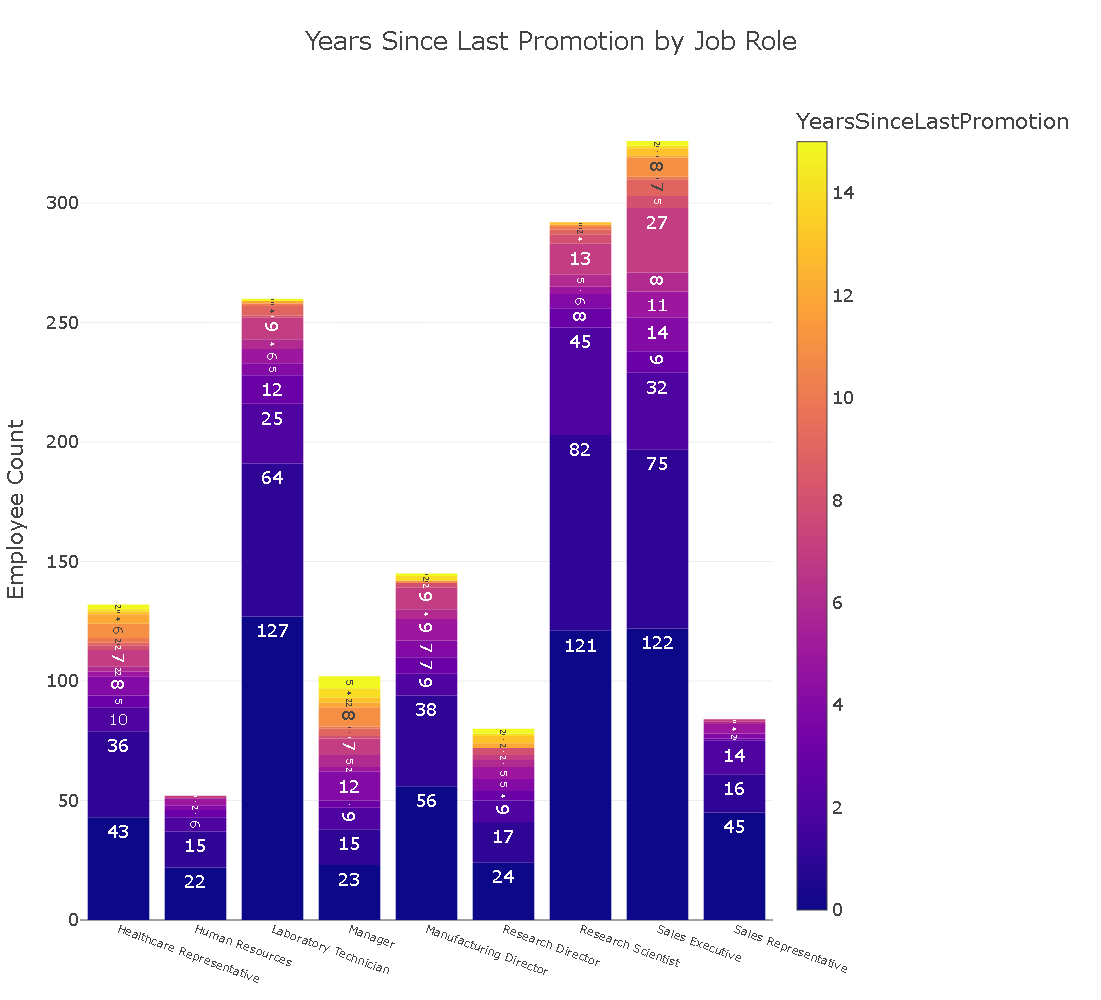
\includegraphics[keepaspectratio]{HR_Analytics_files/figure-pdf/cell-79-output-1.png}}

\subsection{Job Satisfaction by Total Working
Years}\label{job-satisfaction-by-total-working-years}

This stacked bar chart illustrates the relationship between employee job
satisfaction levels and their total years of working experience, helping
to uncover trends across experience levels. Grouping: Aggregates
employee counts based on their job satisfaction level and total working
years.

Visualization: Stacked bars show the distribution of working experience
within each satisfaction level.

Styling: Uses a sequential color palette for smooth gradient and clear
legend.

Exporting: Saves charts as JPG, PNG, and interactive HTML for reporting
and sharing.

This visualization provides insights into how experience may influence
job satisfaction among employees.

\begin{Shaded}
\begin{Highlighting}[]
\NormalTok{exp\_satis }\OperatorTok{=}\NormalTok{ HR\_Analytics\_df.groupby([}\StringTok{\textquotesingle{}JobSatisfaction\textquotesingle{}}\NormalTok{, }\StringTok{\textquotesingle{}TotalWorkingYears\textquotesingle{}}\NormalTok{]).size().reset\_index(name}\OperatorTok{=}\StringTok{\textquotesingle{}count\textquotesingle{}}\NormalTok{)}

\NormalTok{fig }\OperatorTok{=}\NormalTok{ px.bar(}
\NormalTok{    exp\_satis,}
\NormalTok{    x}\OperatorTok{=}\StringTok{\textquotesingle{}JobSatisfaction\textquotesingle{}}\NormalTok{,}
\NormalTok{    y}\OperatorTok{=}\StringTok{\textquotesingle{}count\textquotesingle{}}\NormalTok{,}
\NormalTok{    color}\OperatorTok{=}\StringTok{\textquotesingle{}TotalWorkingYears\textquotesingle{}}\NormalTok{,}
\NormalTok{    title}\OperatorTok{=}\StringTok{\textquotesingle{}Job Satisfaction by Total Working Years\textquotesingle{}}\NormalTok{,}
\NormalTok{    barmode}\OperatorTok{=}\StringTok{\textquotesingle{}stack\textquotesingle{}}\NormalTok{,}
\NormalTok{    text}\OperatorTok{=}\StringTok{\textquotesingle{}count\textquotesingle{}}\NormalTok{,}
\NormalTok{    color\_discrete\_sequence}\OperatorTok{=}\NormalTok{px.colors.sequential.Mint}
\NormalTok{)}

\NormalTok{fig.update\_layout(}
\NormalTok{    template}\OperatorTok{=}\StringTok{\textquotesingle{}presentation\textquotesingle{}}\NormalTok{,}
\NormalTok{    xaxis\_title}\OperatorTok{=}\StringTok{\textquotesingle{}Job Satisfaction Level\textquotesingle{}}\NormalTok{,}
\NormalTok{    yaxis\_title}\OperatorTok{=}\StringTok{\textquotesingle{}Employee Count\textquotesingle{}}\NormalTok{,}
\NormalTok{    legend\_title}\OperatorTok{=}\BuiltInTok{dict}\NormalTok{(text}\OperatorTok{=}\StringTok{\textquotesingle{}Total Working Years\textquotesingle{}}\NormalTok{),}
\NormalTok{    paper\_bgcolor}\OperatorTok{=}\StringTok{"rgba(0,0,0,0)"}\NormalTok{,}
\NormalTok{    plot\_bgcolor}\OperatorTok{=}\StringTok{"rgba(0,0,0,0)"}\NormalTok{,}
\NormalTok{     width}\OperatorTok{=}\DecValTok{900}\NormalTok{,   }
\NormalTok{    height}\OperatorTok{=}\DecValTok{1000}
    
\NormalTok{)}
\NormalTok{fig.update\_traces(textposition}\OperatorTok{=}\StringTok{\textquotesingle{}inside\textquotesingle{}}\NormalTok{)}
\NormalTok{fig.show()}
\NormalTok{fig.write\_image(os.path.join(results\_dir, }\StringTok{\textquotesingle{}job\_satisfaction\_Level.jpg\textquotesingle{}}\NormalTok{))}
\NormalTok{fig.write\_image(os.path.join(results\_dir, }\StringTok{\textquotesingle{}job\_satisfaction\_Level.png\textquotesingle{}}\NormalTok{))}
\NormalTok{fig.write\_html(os.path.join(results\_dir, }\StringTok{\textquotesingle{}job\_satisfaction\_Level.html\textquotesingle{}}\NormalTok{))}
\end{Highlighting}
\end{Shaded}

\pandocbounded{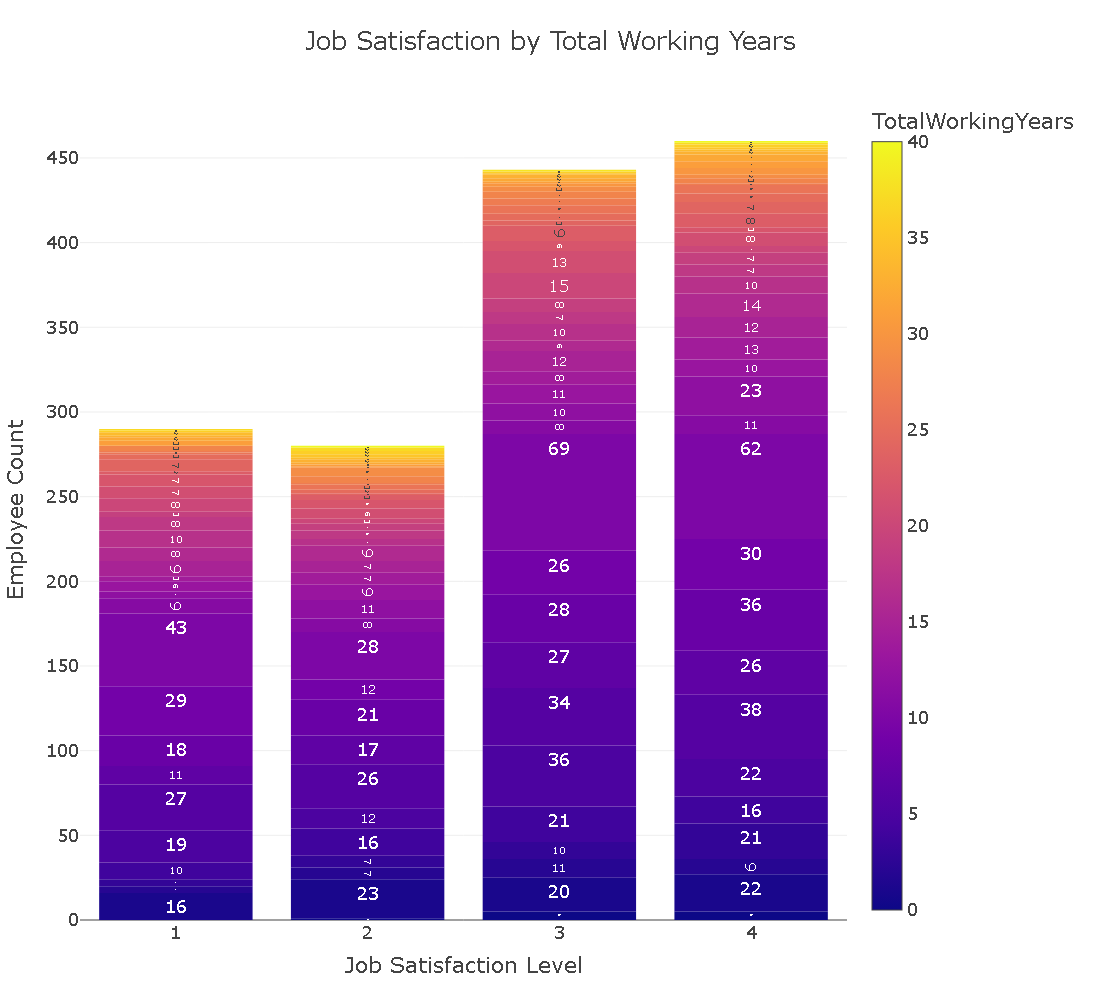
\includegraphics[keepaspectratio]{HR_Analytics_files/figure-pdf/cell-80-output-1.png}}

\section{HR Analytics Project
Summary}\label{hr-analytics-project-summary}

\subsection{Data Cleaning}\label{data-cleaning}

The initial phase involved preparing the HR dataset for analysis by:

\begin{itemize}
\tightlist
\item
  Removing duplicates: Ensured the dataset contains unique records to
  maintain accuracy.
\item
  Renaming columns: Made column names more readable and standardized,
  e.g., renaming \texttt{EnvironmentSatisfaction} to
  \texttt{EnvSatisfaction}.
\item
  Mapping categorical codes to labels: Translated numeric codes into
  meaningful categories for columns like Education, Job Involvement,
  Stock Option Level, Relationship Satisfaction, and Work-Life Balance.
  This improves interpretability.
\item
  Handling missing or irrelevant columns: Dropped unnecessary columns to
  streamline the dataset.
\item
  Saving cleaned data: Exported the cleaned dataset to a CSV file
  (\texttt{Cleaned1.csv}) for further use.
\end{itemize}

This preparation laid a solid foundation for effective and insightful
analysis.

\begin{center}\rule{0.5\linewidth}{0.5pt}\end{center}

\subsection{Data Analysis \&
Visualization}\label{data-analysis-visualization}

Using the cleaned data, multiple visualizations were created to uncover
workforce insights:

\begin{enumerate}
\def\labelenumi{\arabic{enumi}.}
\tightlist
\item
  Attrition Analysis:

  \begin{itemize}
  \tightlist
  \item
    Attrition rates by Job Role, Age Group, and Overtime status to
    identify turnover patterns.
  \item
    Color-coded grouped bar charts highlight which segments have higher
    employee exits.
  \end{itemize}
\item
  Workforce Composition:

  \begin{itemize}
  \tightlist
  \item
    Gender distribution showing diversity within the company.
  \item
    Job Satisfaction levels visualized to assess overall employee
    morale.
  \item
    Average Monthly Income by Job Level to understand compensation
    distribution.
  \item
    Distribution of Job Levels by Education Field to explore career
    progression and educational background.
  \end{itemize}
\item
  Career Development Insights:

  \begin{itemize}
  \tightlist
  \item
    Years Since Last Promotion by Job Role to track advancement trends.
  \item
    Job Satisfaction correlated with Total Working Years to understand
    experience impact on morale.
  \end{itemize}
\end{enumerate}

Each visualization was customized for clarity and impact using Plotly
Express, with thoughtful color schemes and layout settings to enhance
readability. Visuals were exported in JPG, PNG, and interactive HTML
formats for reporting and presentations.

\begin{center}\rule{0.5\linewidth}{0.5pt}\end{center}

\subsubsection{Overall Impact}\label{overall-impact}

The cleaning process ensured data quality and consistency, while the
comprehensive visual analysis provided actionable insights into employee
turnover, satisfaction, compensation, and career growth. This project
equips HR stakeholders with clear, data-driven understanding to inform
retention strategies, career development programs, and diversity
initiatives.

\begin{center}\rule{0.5\linewidth}{0.5pt}\end{center}

Feel free to reach out if you need further analysis, dashboard
integration, or presentation-ready reports




\end{document}
